\documentclass[11pt]{article}

% Change "review" to "final" to generate the final (sometimes called camera-ready) version.
% Change to "preprint" to generate a non-anonymous version with page numbers.
\usepackage{tikz}
\usetikzlibrary{positioning, arrows.meta, calc}

\usepackage{acl}
\usepackage{xurl}
\usepackage{iftex}
\ifPDFTeX
  % pdfLaTeX needs CJKutf8 for the raw Chinese text below.
  \usepackage[T1]{fontenc}
  \usepackage[utf8]{inputenc}
  \usepackage{CJKutf8}
  \usepackage{times}
  \usepackage{microtype}
  \usepackage{inconsolata}
\else
  \usepackage[UTF8,scheme=plain,fontset=fandol]{ctex}
  \setmainfont{TeX Gyre Termes}
  \setmonofont{Inconsolatazi4}[
    BoldFont={Inconsolatazi4-Bold},
    ItalicFont={Inconsolatazi4-Regular},
    BoldItalicFont={Inconsolatazi4-Bold}
  ]
\fi

% Standard package includes
\usepackage{latexsym}
\usepackage{amsmath}
\usepackage{amssymb}
\usepackage{bm}
\usepackage{dsfont}
\usepackage{arydshln}
%Including images in your LaTeX document requires adding
%additional package(s)
\usepackage{graphicx}
\usepackage{adjustbox}
\usepackage{cuted}
\usepackage{booktabs}
\usepackage{siunitx}
\usepackage{multicol}
\usepackage{multirow}
\usepackage{tcolorbox}
\tcbuselibrary{breakable, skins}
\setlength{\emergencystretch}{3em}
\usepackage{xcolor}
\newtcolorbox{PromptBox}[1]{
  colback=gray!5!white,
  colframe=gray!75!black,
  title=#1,
  width=\linewidth,
  sharp corners,
  boxrule=0.8pt,
  fonttitle=\bfseries,
  fontupper=\small,
  enhanced,
  left=1.2mm,
  right=1.2mm,
  top=1.0mm,
  bottom=1.0mm
}


\newcommand{\dashedmidrule}{
  \noalign{\vskip\aboverulesep}
  \hdashline
  \noalign{\vskip\belowrulesep}
}
\setlength{\dashlinedash}{2pt}
\setlength{\dashlinegap}{2pt}

\colorlet{diaggray}{black!60}
\newcommand{\bootcell}[2]{%
  \multicolumn{1}{c}{#1 {\scalebox{0.75}{$\pm$ #2}}}%
}
\newcommand{\diagcell}[2]{%
  \multicolumn{1}{c}{\textcolor{diaggray}{#1 {\scalebox{0.75}{$\pm$ #2}}}}%
}
\sisetup{
  table-format=1.3,
  detect-weight=true,
  explicit-sign=+
}
\newcommand{\nega}[1]{\textcolor{red!70!black}{\num{-#1}}}
\newcommand{\pos}[1]{\textcolor{green!50!black}{\num{+#1}}}


\title{Adaptive Self-Consistency for Long-Form Factuality on Long-Tail Facts}

\author{\textbf{Daniil Moskovskiy\textsuperscript{1,2}}, \textbf{Rafael Grigoryan\textsuperscript{3}},
  \textbf{Evgenii Shuranov\textsuperscript{4}}, \\\textbf{Wenshuai Yin\textsuperscript{5}}, \textbf{and Alexander Panchenko\textsuperscript{2,1}} \\
  \textsuperscript{1}AIRI, \textsuperscript{2}Skoltech, \textsuperscript{3}MSU, \textsuperscript{4}ITMO University, \textsuperscript{5}HSE\\
  \texttt{\href{mailto:A.Panchenko@skol.tech}{A.Panchenko@skol.tech}}}

\begin{document}
\ifPDFTeX
  \begin{CJK*}{UTF8}{gbsn}
\fi
\maketitle
\begin{abstract}
Long-form question answering for rare entities remains challenging for large language models, while inference-time methods for improving factual precision in this setting are underexplored. We study multi-sample self-consistency for long-form generation across various Wikipedia entity popularity tiers using the RiDiC dataset~\citep{braslavski2026chroniclesridicgeneratingdatasets}, using fact-level evaluation. We compare several aggregation strategies and find that LLM-based aggregation consistently outperforms voting and selection baselines, including a compute-matched best-of-$\operatorname{K}$ logprob selector, across languages and domains, with most gains achieved at relatively small sample budgets. Motivated by this early-saturation effect, we introduce an adaptive policy that predicts an appropriate generation budget from pre-generation features. Against a conservative full-budget self-consistency reference (99 generations per question), the adaptive policy retains over 99\% of factual precision while reducing the number of sampled generations by 2--29\% across various language--domain pairs. We further investigate how these savings depend on the reference budget and identify the regime where adaptive routing helps most.
\end{abstract}

\section{Introduction}

Large language models (LLMs) are increasingly used in information-seeking settings that require long, coherent answers rather than short factual snippets. In such settings, factuality failures are especially harmful: long responses may remain fluent and persuasive while still containing multiple unsupported or hallucinated statements~\citep{DBLP:conf/acl/MaynezNBM20,DBLP:journals/csur/JiLFYSXIBMF23}. Long-form factuality is now recognized as a distinct evaluation challenge, since correctness must be assessed over many fine-grained claims rather than a single final answer~\citep{min-etal-2023-factscore,wildhallucinations,DBLP:conf/nips/WeiYSLH0TPLHDL24}. This challenge becomes more severe for unpopular entities, where factual recall is often weaker and purely parametric generation tends to be less reliable~\citep{popqa}. We operationalize popularity using RiDiC's Wikipedia-pageview tiers: ``tail'' denotes low-pageview entities, while head and torso provide higher-popularity comparison groups~\citep{braslavski2026chroniclesridicgeneratingdatasets}.

Self-consistency offers one inference-time remedy: rather than relying on a single sampled response, generate multiple candidate completions and select or synthesize a final answer from them~\citep{self-consistency,universal-self-consistency,thirukovalluru-etal-2024-atomic}. In practice, the saturation point is generally not known in advance since it depends on the task and the model one uses. A conservative large-budget regime is wasteful when most of the gain is realized early. Little is yet known about how to cut this waste for long-form factual generation.

\begin{figure*}
  \centering
  \begin{adjustbox}{trim=1.5cm 0pt 0pt 0pt,clip,width=\textwidth,center}
    % ── Color Palette ───────────────────────────────────────────────────────
\definecolor{neutral_fill}{HTML}{F8F9FA}
\definecolor{neutral_stroke}{HTML}{6B7280}
\definecolor{neutral_title}{HTML}{1F2937}
\definecolor{neutral_sub}{HTML}{4B5563}
\definecolor{amber_fill}{HTML}{FFFBEB}
\definecolor{amber_stroke}{HTML}{D97706}
\definecolor{amber_title}{HTML}{92400E}
\definecolor{amber_sub}{HTML}{B45309}
\definecolor{indigo_fill}{HTML}{EEF2FF}
\definecolor{indigo_stroke}{HTML}{4F46E5}
\definecolor{indigo_title}{HTML}{3730A3}
\definecolor{indigo_sub}{HTML}{4F46E5}
\definecolor{emerald_fill}{HTML}{ECFDF5}
\definecolor{emerald_stroke}{HTML}{059669}
\definecolor{emerald_title}{HTML}{065F46}
\definecolor{emerald_sub}{HTML}{047857}

% ✔ / ✗  symbols
\newcommand{\cmark}{\textcolor{emerald_stroke}{\ensuremath{\checkmark}}}
\newcommand{\xmark}{\textcolor{red!65!black}{\ensuremath{\times}}}
\begin{tikzpicture}[
  >=Stealth, font=\sffamily,
  % ── base box ─────────────────────────────────────────────────────────
  box/.style={rectangle, rounded corners=2.5pt, align=center, inner sep=4pt},
  box_neutral/.style ={box, fill=neutral_fill,  draw=neutral_stroke,  line width=0.5pt},
  box_amber/.style   ={box, fill=amber_fill,    draw=amber_stroke,    line width=1.5pt,
                        minimum height=1.6cm},
  box_indigo/.style  ={box, fill=indigo_fill,   draw=indigo_stroke,   line width=1pt},
  box_emerald/.style ={box, fill=emerald_fill,  draw=emerald_stroke,  line width=0.5pt},
  % ── generation card: left-aligned, small text ────────────────────────
  gen/.style={box, fill=neutral_fill, draw=neutral_stroke, line width=0.4pt,
              text width=2.35cm, align=left, inner sep=3pt},
  % ── arrows ───────────────────────────────────────────────────────────
  arr/.style={-{Stealth[length=4pt,width=3pt]}, line width=1.2pt, draw=#1},
  arr/.default=neutral_stroke,
  % thinner arrows for fan-out/fan-in
  arr_thin/.style={-{Stealth[length=2.8pt,width=2.2pt]},
                   line width=0.7pt, draw=neutral_stroke!70},
  dashline/.style={densely dashed, line width=0.4pt, draw=neutral_sub!60}
]

%% ── (1) Input ──────────────────────────────────────────────────────────
\node[box_neutral, text width=2.2cm, inner sep=3pt] (inp) {
  \textbf{\color{neutral_title}Input}\\[2pt]
  {\scriptsize\color{neutral_sub}
   ``Tell me about\\the Jordan River''}
};

%% ── (2) Sampling ───────────────────────────────────────────────────────
\node[box_neutral, anchor=west] (sam)
  at ($(inp.east)+(1.0cm,0)$) {
  \textbf{\color{neutral_title}Sampling}\\[2pt]
  {\small\color{neutral_sub}(Self-Consistency)}
};

%% ── (3) Generation cards  y¹ y² y³ ────────────────────────────────────
% placed as a vertical column to the right of Sampling
\node[gen, anchor=west] (y1) at ($(sam.east)+(1.0cm,+1.2cm)$) {
  % {\scriptsize\textbf{\color{neutral_title}$y^1$}}\\[-3pt]
  {\tiny \cmark\ 251\,km long}\\[-4pt]
  {\tiny \xmark\ origin: Turkey}\\[-4pt]
  {\tiny \cmark\ flows into the Dead Sea}
};

\node[gen, anchor=west] (y2) at ($(sam.east)+(1.0cm,0)$) {
  % {\scriptsize\textbf{\color{neutral_title}$y^2$}}\\[-3pt]
  {\tiny \xmark\ 350\,km long}\\[-4pt]
  {\tiny \cmark\ flows into the Dead Sea}\\[-4pt]
  {\tiny \cmark\ sacred in 3\,religions}
};

\node[gen, anchor=west] (y3) at ($(sam.east)+(1.0cm,-1.2cm)$) {
  % {\scriptsize\textbf{\color{neutral_title}$y^3$}}\\[-3pt]
  {\tiny \cmark\ 251\,km long}\\[-4pt]
  {\tiny \xmark\ flows into Med.\ Sea}\\[-4pt]
  {\tiny \cmark\ sacred in 3\,religions}
};

% optional: light bounding box around the three cards
\draw[dashline, rounded corners=3pt]
  ($(y1.north west)+(-0.12cm,+0.18cm)$)
  rectangle
  ($(y3.south east)+(+0.12cm,-0.18cm)$);

%% ── (4) LLM Aggregation ────────────────────────────────────────────────
\node[box_amber, anchor=west, text width=2.8cm] (agg)
  at ($(y2.east)+(1.0cm,0)$) {
  \textbf{\color{amber_title}LLM aggregation}\\[2pt]
  {\small\color{amber_sub}(LLMAgg)}\\[2pt]
  {\small$\hat{y}=A(y^1,\dots,y^K)$}
};

%% ── (5) Output ─────────────────────────────────────────────────────────
\node[box_neutral, anchor=west, text width=3.0cm, inner sep=3pt] (out)
  at ($(agg.east)+(1.0cm,0)$) {
  \textbf{\color{neutral_title}Output}\\[2pt]
  {\color{neutral_sub}\parbox[t]{2.8cm}{\scriptsize\centering
   The Jordan River (251\,km) flows from Lebanon-Syria into the Dead Sea.
   It is sacred in Jewish, Christian, and Islamic traditions.}}
};

%% ── (6) FactOWL ────────────────────────────────────────────────────────
\node[box_emerald, anchor=west] (fact)
  at ($(out.east)+(0.9cm,0)$) {
  \textbf{\color{emerald_title}FactOWL}\\[2pt]
  {\small\color{emerald_sub}fact-level score}
};

%% ── Adaptive Sampling ──────────────────────────────────────────────────
% anchored by its north so the gap below sam.south is exact
\node[box_indigo, anchor=north] (ada)
  at ($(sam.south)+(0,-2.4cm)$) {
  \textbf{\color{indigo_title}Adaptive Sampling}\\[2pt]
  {\small\color{indigo_sub}$g(x)\to\text{predicted }K$}
};

%% ── Main pipeline arrows ───────────────────────────────────────────────
\draw[arr] (inp.east)  -- (sam.west);
\draw[arr] (agg.east)  -- (out.west);
\draw[arr] (out.east)  -- (fact.west);

%% ── Fan-out: Sampling → y¹ y² y³ ──────────────────────────────────────
\draw[arr_thin] (sam.east) to[out=0, in=180] (y1.west);
\draw[arr_thin] (sam.east) --                (y2.west);
\draw[arr_thin] (sam.east) to[out=0, in=180] (y3.west);

%% ── Fan-in: y¹ y² y³ → LLMAgg ─────────────────────────────────────────
\draw[arr_thin] (y1.east) to[out=0, in=150] (agg.west);
\draw[arr_thin] (y2.east) --                (agg.west);
\draw[arr_thin] (y3.east) to[out=0, in=210] (agg.west);

%% ── Adaptive arrows ────────────────────────────────────────────────────
\draw[arr={indigo_stroke}]
  (ada.north) -- node[left, font=\small, text=indigo_sub] {$K$} (sam.south);

% L-shaped: inp.south ↓ then → ada.west
\draw[arr] (inp.south) |- (ada.west);

%% ── Annotations ────────────────────────────────────────────────────────

% below LLMAgg
\draw[dashline] (agg.south) -- ++(0,-0.38) coordinate (mid);
\node[font=\scriptsize, text=neutral_sub, align=center, text width=3.0cm]
  at ($(mid)+(0,-0.26)$)
  {merge consistent facts\\remove contradictions};

% right of Adaptive Sampling
\node[font=\scriptsize, text=neutral_sub, align=left, text width=2.8cm,
      anchor=west]
  at ($(ada.east)+(0.38cm,0)$)
  {Hard inputs$\to$large $K$\\Easy inputs$\to$small$K$};

\end{tikzpicture}

  \end{adjustbox}
  \caption{Overview of the proposed pipeline. An input prompt is sampled multiple times via self-consistency. An adaptive controller predicts the generation budget $\operatorname{K}$ from the input features. Candidate generations are aggregated via LLMAgg, and the final output is assessed with fact-level evaluation.}
  \label{fig:pipeline}
\end{figure*}

Studying this setting requires an evaluation protocol that combines long-form generation, fact-level verification, multilingual coverage, domain diversity, and explicit Wikipedia-pageview popularity tiers. Existing resources satisfy these requirements only partially. Benchmarks with popularity annotations, such as PopQA, are centered on short-answer question answering rather than long-form generation~\citep{popqa}. Long-form factuality benchmarks better match the generation setting~\citep{min-etal-2023-factscore, wildhallucinations}, but they often do not provide controlled popularity strata or domain splits, making it harder to isolate long-tail effects~\citep{wildhallucinations, DBLP:conf/nips/WeiYSLH0TPLHDL24, vazhentsev2026leveragingllmparametricknowledge}. We therefore evaluate on the existing RiDiC benchmark, whose entity-centric prompts, multilingual coverage, domain splits, and Wikipedia-pageview tiers support this controlled analysis~\citep{braslavski2026chroniclesridicgeneratingdatasets}.

We ask three questions: (i) whether multi-sample self-consistency improves long-form factual precision across these popularity tiers, (ii) which aggregation strategy best consolidates multiple long-form generations, and (iii) how much of the factuality gain survives when the sampling budget is allocated adaptively rather than fixed at the full-budget reference.

Our contributions are empirical rather than a new benchmark or factuality evaluator: (i) we compare content-level LLM aggregation with selection and voting baselines for long-form factuality on RiDiC; (ii) we characterize budget--factuality curves across languages, domains, and popularity tiers; and (iii) we evaluate a lightweight pre-generation policy that routes inputs to a sampling budget relative to a conservative full-budget reference.

Within this single-generator setting, LLMAgg substantially outperforms single generation, voting baselines, and a compute-matched best-of-$\operatorname{K}$ logprob selector across domains and languages. The budget-scaling curves saturate early but vary across domains and languages. We therefore add a simple routing policy that predicts the generation budget before candidate generation. Against the full-budget reference, the policy retains nearly all factual precision while reducing the number of sampled generations.

\section{Related Work}

\paragraph{Self-Consistency} improves language-model reliability by sampling multiple outputs and aggregating them~\citep{self-consistency}. Most prior work studies this idea in reasoning and short-answer settings, where aggregation can often be reduced to voting over final answers. Universal Self-Consistency extends the paradigm to open-ended generation through response selection~\citep{universal-self-consistency}, while Atomic Self-Consistency aggregates selected atomic subparts of candidate generations~\citep{thirukovalluru-etal-2024-atomic}.

Our setting differs from these scenarios. Long-form generations contain many partially correct and partially incorrect statements, so agreement at the response level is a weak proxy for factual correctness. Aggregation strategies can also behave very differently when candidates overlap without being identical. We therefore study aggregation directly, comparing LLM-based aggregation against selection and voting baselines under fact-level evaluation.

\paragraph{Long-Form Factuality Evaluation}

Long-form factuality is now treated as a distinct evaluation problem, because generated responses often contain many atomic claims whose correctness must be assessed individually rather than through exact-match style metrics~\citep{DBLP:conf/acl/MaynezNBM20, min-etal-2023-factscore, DBLP:journals/csur/JiLFYSXIBMF23}. FActScore formalizes this perspective by decomposing long-form outputs into atomic facts and measuring the fraction that can be supported~\citep{min-etal-2023-factscore}. Other recent benchmarks, such as WildHallucinations~\citep{wildhallucinations}, further emphasize the difficulty of maintaining factual consistency in entity-centric long-form generation.

These benchmarks establish the need for fact-level evaluation, but they only partially match the setting we study here. Popularity-aware resources such as PopQA target short-answer factual recall rather than long-form generation~\citep{popqa}, while long-form factuality benchmarks do not always provide controlled popularity partitions together with multilingual and domain-structured evaluation. Our work builds on this literature by studying inference-time factuality across pageview-defined popularity tiers.

\begin{figure*}
  \centering
  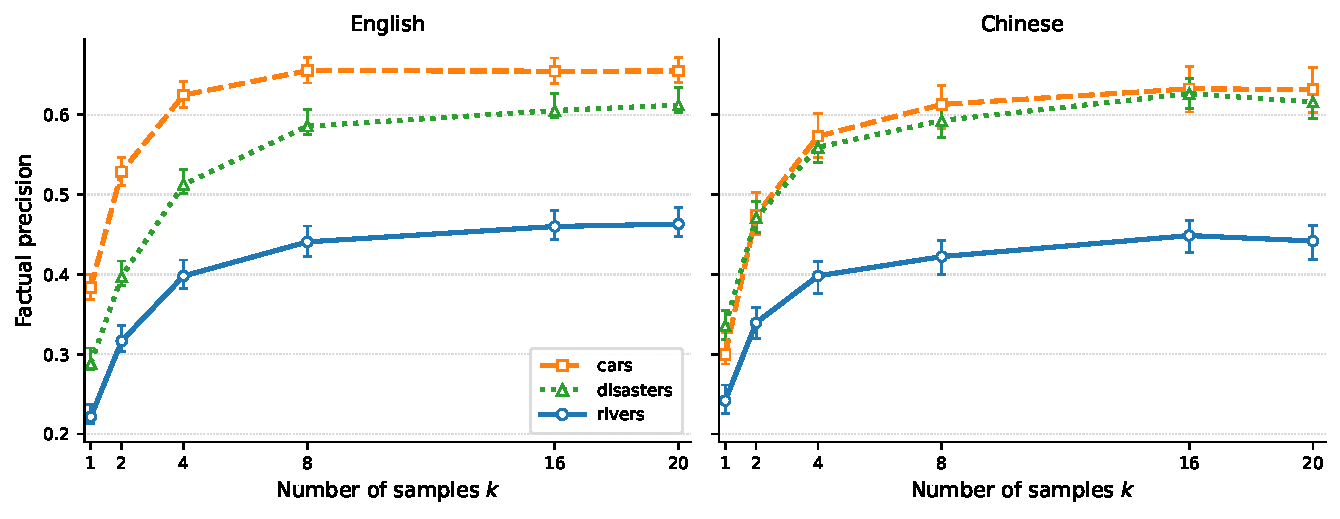
\includegraphics[clip,width=\textwidth]{figures/prefix_scaling_en_zh.pdf}%
  \caption{LLMAgg budget-scaling curves across sample budgets. Performance improves sharply at small $\operatorname{K}$ and saturates by roughly $\operatorname{K}\!=\!8$--$16$ in both languages, with only marginal changes beyond $\operatorname{K}\!=\!20$. The saturation point is heterogeneous across domains, which motivates input-conditioned routing rather than a single fixed budget.}
  \label{fig:prefix_scaling}
\end{figure*}

\paragraph{Adaptive Inference and Test-Time Scaling}

Recent work shows that additional inference-time computation can improve model outputs. Test-time scaling results suggest that increasing the number of samples can substantially improve performance, in some cases more effectively than scaling model size alone~\citep{snell2024scalingllmtesttimecompute, Wu2024InferenceSL}. These gains, however, are heterogeneous across inputs. Adaptive methods respond by allocating more compute only where it is expected to help.

This idea was explored in self-consistency and confidence-aware inference, including early-stopping and reliability-aware variants of multi-sample decoding~\citep{taubenfeld2025confidence, reasc, marina-etal-2026-boosting}. We take the same perspective but target long-form factual generation evaluated at the level of atomic claims. In this setting, the main question is not only whether more samples help, but how much of the aggregation gain can be preserved when the sampling budget is routed adaptively relative to a conservative full-budget reference.

\section{Method}

We combine self-consistency, LLM-based aggregation, and adaptive inference into a compute-aware framework for long-form factuality. Given an input prompt $x$, we generate multiple candidate responses, aggregate them into a single output, and evaluate factuality at the level of individual facts. Figure~\ref{fig:pipeline} illustrates the overall pipeline.

\paragraph{Self-Consistency Sampling}

Given an input prompt $x$, we sample $\operatorname{K}$ independent responses:
\[
y^{(1)}, y^{(2)}, \dots, y^{(\operatorname{K})} \sim p_\theta(y \mid x).
\]

This diversity is what lets us identify factual information that is consistent across samples. Unlike standard single-generation inference, self-consistency allows the model to explore multiple plausible answers, some of which may correct errors present in others.

\paragraph{LLM-based Aggregation}

To obtain a final response, we aggregate the sampled outputs using an LLM-based aggregation function (LLMAgg):
\[
\hat{y} = \mathcal{A}(y^{(1)}, \dots, y^{(\operatorname{K})}).
\]

The aggregation model is prompted to merge consistent factual statements across samples while removing contradictions and unsupported claims. This step leverages redundancy in the sampled outputs to improve factual precision.

As shown in Figure~\ref{fig:pipeline}, aggregation operates on multiple sampled responses. Unlike majority voting or heuristic selection, LLMAgg works on the text itself, so it can merge complementary facts from different generations.

\begin{figure*}
  \centering
  \IfFileExists{figures/adaptive_feature_importance.pdf}{%
    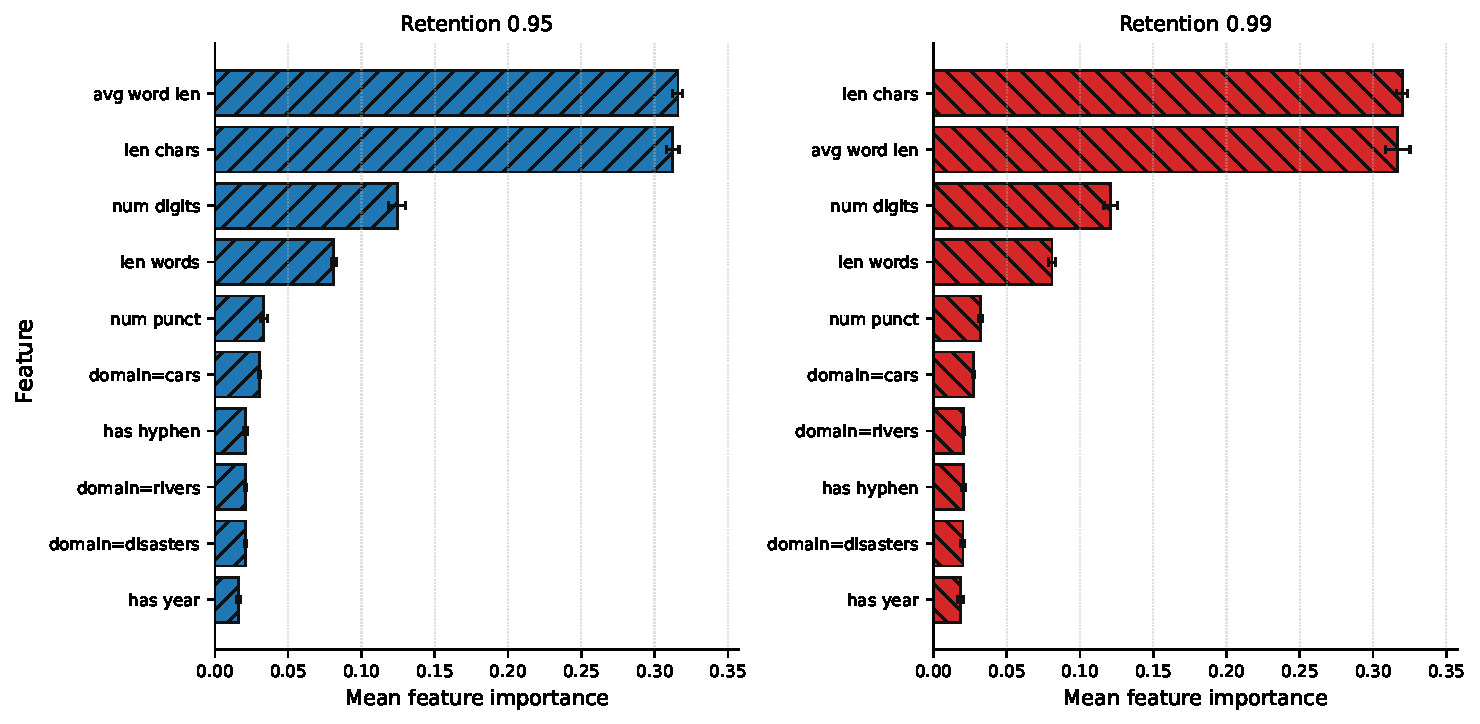
\includegraphics[clip, trim=0.25cm 0cm 0cm 0cm, width=\textwidth]{figures/adaptive_feature_importance.pdf}%
  }{%
    \fbox{\parbox{0.92\textwidth}{\centering Adaptive feature-importance figure placeholder.}}%
  }
  \caption{Feature importance for the adaptive controller. Input length and lexical-complexity features dominate, while language and domain indicators contribute relatively little. Error bars show the standard deviation of feature importance across runs.}
  \label{fig:feature_importance}
\end{figure*}

\paragraph{Adaptive Sampling}

Instead of using a fixed full-budget number of samples $\operatorname{K}_{\text{full}}$, we employ an adaptive strategy that predicts a generation budget for each input:
$\operatorname{K}\!=\!g(x),$
where $g$ is a lightweight classifier designed to approximate the marginal benefit of additional sampling.

Different inputs have different levels of factual uncertainty. For difficult inputs, more samples increase the chance of observing correct facts, while for easier inputs, fewer samples are sufficient. Because the saturation point is heterogeneous across domains and not known before evaluation, an input-conditioned policy can reduce reliance on a single conservative budget within the evaluated distribution.

The result is a cost–factuality trade-off that spends extra samples only where they are needed.

\section{Experimental Setup}

\paragraph{Dataset}

Evaluating long-form factuality across pageview-defined popularity tiers requires more than a standard entity benchmark. Popularity-aware resources such as PopQA provide valuable supervision for knowledge frequency, but they target short-answer question answering rather than long-form generation~\citep{popqa}. Long-form factuality benchmarks are closer to our setting, but they typically do not provide explicit domain splits together with controlled popularity partitions, which limits their usefulness for analyzing long-tail behavior in a structured way~\citep{wildhallucinations}.

We use RiDiC~\citep{braslavski2026chroniclesridicgeneratingdatasets}, an existing benchmark for entity-centric long-form factuality evaluation with explicit popularity stratification. RiDiC covers three domains (rivers, cars, and disasters) and two languages (English and Chinese). The nominal test split contains 1000 examples per domain. We use its public test metadata and the corresponding public self-consistency exports and their Chinese counterparts.\footnote{\url{hf.co/datasets/s-nlp/RiDiC_rivers_self_consistency_99_generations}}$^,$\footnote{
\url{hf.co/datasets/s-nlp/RiDiC\_cars\_self\_consistency\_99\_generations}}$^,$\footnote{\url{hf.co/datasets/s-nlp/RiDiC\_bad\_weather\_self\_consistency\_99\_generations}}
After filtering for usable entity titles and Wikipedia contexts, the effective counts are $1000/997/1000$ for English rivers/cars/disasters and $723/400/723$ for the corresponding Chinese cells. Table~\ref{tab:ridicexample} presents an example from the RiDiC benchmark, illustrating the variability and factual inconsistencies in model outputs.

Thus, \texttt{test}~\texttt{split} refers to the public test partition; reported FactOWL scores use the usable-context subset of that partition. Its \texttt{head}, \texttt{torso}, and \texttt{tail} tiers are derived from the \texttt{popularity\_part\_sector}, which is based on Wikipedia page views. We use this stratification as an analysis axis: it reveals whether factuality and budget behavior persist under the benchmark's controlled variation in entity popularity.

\paragraph{Generation}

We use Llama 3.1 8B Instruct~\citep{llama3} with stochastic decoding to induce diversity across generations. The same generator is used for English and Chinese to hold model capacity fixed across the language comparison; we do not claim language-equivalent performance. The saved exports were generated before this study, and their original temperature/top-$p$ settings are not recorded in the available artifacts; consequently, we do not claim to reproduce those decoding parameters here. For the scoring and aggregation reruns, we use vLLM in bfloat16 with tensor parallelism set to $1$, GPU memory utilization $0.8$, model seed $0$, and the maximum of $256$ generated tokens. LLMAgg is a separate call to the same Llama checkpoint, with temperature 0 and maximum 256 new tokens; it is not the generator's original completion call. In the full self-consistency setting, we use the available 99 candidate completions per input and set $\operatorname{K}_{\text{full}}=99$ as a conservative full-budget reference. Budget-scaling curves use nested prefixes, meaning the first $\operatorname{K}$ candidates from this fixed ordered pool, for $\operatorname{K}\!\in\!\{1,2,4,8,16,20\}$; no new sampling is performed at each curve point. Decoding and prompt settings are held fixed across rerun methods.


\begin{table*}
\small
\centering
\begin{tabular}{p{0.95\textwidth}}
\toprule
\textbf{Entity:} Xiaomi SU7 \\
\midrule

\textbf{Model Output A (hallucinated):}
The Xiaomi SU7 is a subcompact SUV based on the SAIC MG ZS platform,
featuring a 1.5-liter engine and manual transmission. \\

\textbf{Model Output B (partially correct):}
The Xiaomi SU7 is an electric SUV launched in 2022, offering a range
of up to 600 km and competing with vehicles such as the Tesla Model Y. \\

\textbf{Model Output C (more accurate):}
The Xiaomi SU7 is an all-electric sedan unveiled in 2023, built on
Xiaomi's proprietary platform, with high-performance variants exceeding
600 horsepower and long driving range. \\

\midrule

\textbf{Example Facts:}
\begin{itemize}
    \item The Xiaomi SU7 is an electric vehicle. \hfill (True)
    \item It is a subcompact SUV based on MG ZS. \hfill (False)
    \item It was unveiled in 2023. \hfill (True)
    \item It has a 1.5L combustion engine. \hfill (False)
    \item It competes with Tesla Model Y. \hfill (Partially True)
\end{itemize}
\\
\bottomrule
\end{tabular}
\caption{Example from RiDiC showing inconsistent generations for the same entity.}
\label{tab:ridicexample}
\end{table*}

\paragraph{Compared Methods}

We report six conditions in Table~\ref{tab:results}. \textbf{Single} uses one generated completion and performs no aggregation. \textbf{Best samp.} is a non-deployable diagnostic that selects the factuality-best individual candidate after scoring. \textbf{MC} (majority co-occurrence) is a response-level agreement baseline: it votes on whether a candidate is supported rather than decomposing responses into facts. \textbf{MF} performs majority fact-level voting over normalized FactOWL-derived atomic facts; an atom is retained when it occurs in at least $\lceil \frac{\operatorname{K}}{2}\rceil$ candidate responses, and its saved support decision is the majority of its FactOWL decisions. \textbf{SP} (SeqProb) is a selector that scores each candidate by its mean token log-probability under the same Llama generator and chooses the highest-scoring candidate. \textbf{LLMAgg} uses a separate, deterministic-temperature Llama call to synthesize a final response from multiple candidates. Unlike selection-based methods, it can combine information across generations rather than choosing a single candidate. The compute-matched \textbf{Best-of-$\operatorname{K}$ logprob} selector chooses the candidate with the highest average token logprob from the same 20-sample pool as LLMAgg@$\operatorname{K}{=}20$. We report that matched $\operatorname{K}{=}20$ comparison in Appendix~\ref{app:baselines}, rather than Table~\ref{tab:results}, which reports the full-budget LLMAgg@$\operatorname{K}{=}99$ comparison.

\paragraph{Evaluation}

We use FactOWL\footnote{\url{https://github.com/s-nlp/factowl}}~\citep{factowl} as a fact-level evaluation framework that decomposes long-form outputs into atomic claims and estimates factual precision from their support status. In our configuration, the Llama 3.1 8B Instruct model performs both atomic-fact generation and fact verification, with temperature 0, a $256\!-$token generation limit for atomic-fact extraction, and an $8-$token verification output limit. Using the same model as both extractor and verifier follows a broader practice of treating LLMs as annotators of textual properties, from toxicity labels to factual support~\citep{moskovskiy-etal-2024-llms, pletenev-etal-2025-much}. Verification uses the entity's supplied Wikipedia page as context through the \texttt{retrieval+llama} configuration; the pipeline does not query an alternative evidence corpus for these scores. Each extracted fact is mapped to a binary support decision, and the response score is the mean support indicator over its extracted facts.

We report factual precision as the main metric. Coverage and retention curves are computed from per-topic scoring outputs. In the main results, \textbf{Single} is an independently sampled one-generation baseline, whereas $\operatorname{K}=1$ denotes the first nested prefix of the self-consistency candidate pool; they are therefore not expected to match exactly. Because \textbf{Best samp.} is restricted to individual sampled candidates whereas LLMAgg writes a new response from the pool, it is a diagnostic rather than an upper bound on LLMAgg. This comparison measures factual precision, not recall: by combining supported claims from different candidates and omitting unsupported ones, LLMAgg can produce a response with a higher fraction of supported claims than any individual candidate.

\paragraph{Uncertainty Estimation}

We estimate uncertainty with nonparametric bootstrap confidence intervals for the main metrics. For each setting, we resample test instances with replacement 1000 times and compute percentile 95\% confidence intervals for factual precision, sampled-generation savings, and score retention. We do not perform a separate pairwise significance test; the intervals are descriptive uncertainty estimates and are not interpreted as formal hypothesis-test results.

\paragraph{Adaptive Policy}

To reduce sampled-generation cost relative to the full-budget reference, we train a random-forest classifier that predicts an appropriate generation budget from the allowed curve values. The classifier uses $300$ trees, minimum leaf size $3$, balanced-subsample class weighting, and seed $13$. Features include prompt character/word/token lengths, average word length, digit and punctuation counts, year and question-marker indicators, language and domain indicators, and a domain-level budget prior derived from the budget-scaling curves. Full feature definitions are given in Appendix~\ref{app:features}. We use five stratified shuffle splits with a $30$\% test fraction for the multilingual policy; each fold uses the same split seed $13$ and model seed $13$ plus the fold index. The policy is pre-generation: it uses no partial output, model-confidence, or inter-candidate-disagreement feature. Feature importance is dominated by input length (about $0.31$) and average word length (about $0.32$), while domain and language features contribute less than $0.03$. This indicates that the policy relies primarily on input complexity rather than domain identity.

We intentionally use a simple model to isolate whether pre-generation signals alone are sufficient to capture variation in required compute relative to the full-budget reference.

We report two operating points, corresponding to retention targets of $0.95$ and $0.99$. These are interpretable practical tolerances: allowing at most $5$\% or $1$\% loss relative to the reference. They are operating points rather than statistically optimized thresholds. We define \texttt{compute\_savings} as the relative reduction in sampled generations with respect to the full-budget LLMAgg reference at $\operatorname{K}_{\text{full}}=99$, \texttt{score\_retention} as $\mathrm{Fact}(\hat{y}_{\text{adaptive}}) / \mathrm{Fact}(\hat{y}_{\text{full}})$, and \texttt{coverage} as the fraction of examples meeting the retention target.

\section{Results}

% \begin{table*}[htbp!]
% \centering
% \footnotesize
% % локальное переопределение: ± std теперь в 0.75 от размера таблицы (footnotesize)
% \renewcommand{\bootcell}[2]{%
%   \multicolumn{1}{c}{#1 {\scalebox{0.75}{$\pm$ #2}}}%
% }
% % \setlength{\tabcolsep}{2pt}
% %\begin{adjustbox}{max width=\textwidth,center}
% \begin{tabular}{
% l l
% S[table-format=1.3]
% S[table-format=1.3]
% S[table-format=1.3]
% S[table-format=1.3]
% S[table-format=1.3]
% S[table-format=1.3]
% }
% \toprule
% \textbf{Lang} & \textbf{Domain} &
% \textbf{Single} & \textbf{Best samp.} &
% \textbf{MC} & \textbf{MF} &
% \textbf{SP} & \textbf{LLMAgg (Ours)} \\
% \midrule

% \multirow{3}{*}{EN}
%  & rivers     & \bootcell{0.211}{0.012} & \bootcell{0.450}{0.015} & \bootcell{0.053}{0.014} & \bootcell{0.088}{0.008} & \multicolumn{1}{c}{0.233} & \multicolumn{1}{c}{\textbf{0.465} {\scalebox{0.75}{$\pm$ 0.019}}} \\
%  & cars       & \bootcell{0.344}{0.014} & \bootcell{0.622}{0.013} & \bootcell{0.218}{0.026} & \bootcell{0.146}{0.012} & \multicolumn{1}{c}{0.412} & \multicolumn{1}{c}{\textbf{0.656} {\scalebox{0.75}{$\pm$ 0.016}}} \\
%  & disasters  & \bootcell{0.283}{0.012} & \bootcell{0.574}{0.012} & \bootcell{0.112}{0.020} & \bootcell{0.111}{0.010} & \multicolumn{1}{c}{0.352} & \multicolumn{1}{c}{\textbf{0.619} {\scalebox{0.75}{$\pm$ 0.015}}} \\
% \multicolumn{2}{l}{\textbf{EN macro avg.}} & \multicolumn{1}{c}{0.279} & \multicolumn{1}{c}{0.549} & \multicolumn{1}{c}{0.128} & \multicolumn{1}{c}{0.115} & \multicolumn{1}{c}{0.332} & \multicolumn{1}{c}{\textbf{0.580}} \\
% \midrule

% \multirow{3}{*}{ZH}
%  & rivers     & \bootcell{0.266}{0.018} & \bootcell{0.555}{0.019} & \bootcell{0.154}{0.027} & \bootcell{0.034}{0.007} & \multicolumn{1}{c}{0.233} & \multicolumn{1}{c}{\textbf{0.440} {\scalebox{0.75}{$\pm$ 0.021}}} \\
%  & cars       & \bootcell{0.344}{0.021} & \bootcell{0.640}{0.022} & \bootcell{0.216}{0.040} & \bootcell{0.019}{0.006} & \multicolumn{1}{c}{0.412} & \multicolumn{1}{c}{\textbf{0.632} {\scalebox{0.75}{$\pm$ 0.029}}} \\
%  & disasters  & \bootcell{0.355}{0.018} & \bootcell{0.707}{0.014} & \bootcell{0.234}{0.029} & \bootcell{0.031}{0.007} & \multicolumn{1}{c}{0.352} & \multicolumn{1}{c}{\textbf{0.616} {\scalebox{0.75}{$\pm$ 0.020}}} \\
% \multicolumn{2}{l}{\textbf{ZH macro avg.}} & \multicolumn{1}{c}{0.322} & \multicolumn{1}{c}{0.634} & \multicolumn{1}{c}{0.201} & \multicolumn{1}{c}{0.028} & \multicolumn{1}{c}{0.332} & \multicolumn{1}{c}{\textbf{0.563}} \\
% \bottomrule
% \end{tabular}%
% %\end{adjustbox}
% \caption{Performance comparison across languages and domains. Cells show bootstrap mean $\pm$ half-width for methods with topic-level traces; \textbf{SP} is summary-only and has no bootstrap trace. Macro rows average the displayed domain means and therefore omit intervals. Bold marks the strongest deployable condition. \textbf{Single}: one generation, no aggregation. \textbf{Best samp.}: factuality-best individual candidate, a non-deployable diagnostic. \textbf{MC}: response-level majority co-occurrence voting. \textbf{MF}: majority fact-level voting. \textbf{SP}: SeqProb selection. \textbf{LLMAgg}: LLM-based aggregation ($\operatorname{K}\!=\!99$).
%     }
% \label{tab:results}
% \end{table*}

\begin{table*}
\centering
\footnotesize
% \setlength{\tabcolsep}{2pt}
%\begin{adjustbox}{max width=\textwidth,center}
\begin{tabular}{
l l
S[table-format=1.3]
S[table-format=1.3]
S[table-format=1.3]
S[table-format=1.3]
S[table-format=1.3]
S[table-format=1.3]
}
\toprule
\textbf{Lang} & \textbf{Domain} & 
\textbf{Single} & \textcolor{diaggray}{\textbf{Best samp.}} &
\textbf{MC} & \textbf{MF} & 
\textbf{SP} & \textbf{LLMAgg} \\
\midrule

\multirow{3}{*}{EN}
 & rivers     & \bootcell{0.211}{0.012} & \diagcell{0.450}{0.015} & \bootcell{0.053}{0.014} & \bootcell{0.088}{0.008} & \multicolumn{1}{c}{0.233} & \multicolumn{1}{c}{\textbf{0.462} {\scalebox{0.75}{$\pm$ 0.019}}} \\
 & cars       & \bootcell{0.344}{0.014} & \diagcell{0.622}{0.013} & \bootcell{0.218}{0.026} & \bootcell{0.146}{0.012} & \multicolumn{1}{c}{0.412} & \multicolumn{1}{c}{\textbf{0.653} {\scalebox{0.75}{$\pm$ 0.016}}} \\
 & disasters  & \bootcell{0.283}{0.012} & \diagcell{0.574}{0.012} & \bootcell{0.112}{0.020} & \bootcell{0.111}{0.010} & \multicolumn{1}{c}{0.352} & \multicolumn{1}{c}{\textbf{0.620} {\scalebox{0.75}{$\pm$ 0.015}}}  \\
\textbf{EN} & macro avg. & \multicolumn{1}{c}{0.279} & \multicolumn{1}{c}{\textcolor{diaggray}{0.549}} & \multicolumn{1}{c}{0.128} & \multicolumn{1}{c}{0.115} & \multicolumn{1}{c}{0.332} & \multicolumn{1}{c}{\textbf{0.578}} \\
\midrule

\multirow{3}{*}{ZH}
 & rivers     & \bootcell{0.266}{0.018} & \diagcell{0.555}{0.019} & \bootcell{0.154}{0.027} & \bootcell{0.034}{0.007} & \multicolumn{1}{c}{0.310} & \multicolumn{1}{c}{\textbf{0.451} {\scalebox{0.75}{$\pm$ 0.021}}} \\
 & cars       & \bootcell{0.344}{0.021} & \diagcell{0.640}{0.022} & \bootcell{0.216}{0.040} & \bootcell{0.019}{0.006} & \multicolumn{1}{c}{0.417} & \multicolumn{1}{c}{\textbf{0.632} {\scalebox{0.75}{$\pm$ 0.029}}} \\
 & disasters  & \bootcell{0.355}{0.018} & \diagcell{0.707}{0.014} & \bootcell{0.234}{0.029} & \bootcell{0.031}{0.007} & \multicolumn{1}{c}{0.455} & \multicolumn{1}{c}{\textbf{0.631} {\scalebox{0.75}{$\pm$ 0.020}}} \\
\textbf{ZH} & macro avg. & \multicolumn{1}{c}{0.322} & \multicolumn{1}{c}{\textcolor{diaggray}{0.634}} & \multicolumn{1}{c}{0.201} & \multicolumn{1}{c}{0.028} & \multicolumn{1}{c}{0.394} & \multicolumn{1}{c}{\textbf{0.571}} \\
\bottomrule
\end{tabular}

\caption{Performance comparison across languages and domains. Cells show bootstrap mean $\pm$ half-width for methods with topic-level traces; \textbf{SP} is summary-only and has no bootstrap trace. Macro rows average the displayed domain means and therefore omit intervals. Bold marks the strongest deployable condition; \textcolor{diaggray}{grayed-out values} are oracle diagnostics excluded from the comparison. \textbf{Single}: one generation, no aggregation. \textcolor{diaggray}{\textbf{Best samp.}}: factuality-best individual candidate, a non-deployable diagnostic. \textbf{MC}: response-level majority co-occurrence voting. \textbf{MF}: majority fact-level voting. \textbf{SP}: SeqProb selection. \textbf{LLMAgg}: LLM-based aggregation ($\operatorname{K}\!=\!99$).}
\label{tab:results}
\end{table*}



% The central result is that aggregation, rather than sampling alone, is the main driver of factuality gains in this setting. Across all language--domain combinations, LLMAgg is the strongest method overall, consistently outperforming the raw single-sample baseline as well as weaker selection and voting alternatives.

% Two conclusions follow from Table~\ref{tab:results}. First, multi-sample inference is useful only when the sampled candidates are combined with a sufficiently strong aggregation mechanism. Selection-based baselines such as SeqProb improve over Single, but they remain substantially weaker than LLMAgg. The same conclusion holds for a compute-matched best-of-$\operatorname{K}$ logprob selector evaluated on the same 20-sample pool: it improves over Single in every cell but still trails LLMAgg by 0.14--0.29 factual-precision points (see Appendix~\ref{app:baselines} for details). Likewise, majority-style aggregation over completions or fact decisions fails to recover the same gains. This indicates that long-form factuality benefits less from choosing one ``best'' candidate than from consolidating partially correct information distributed across several candidates.

% Second, LLMAgg is robust across heterogeneous settings rather than being driven by a single favorable slice of the benchmark. The same ordering of methods recurs across both languages and all three domains, despite substantial differences in absolute difficulty. In English, LLMAgg even matches or exceeds the oracle best individual candidate in the sampled pool, which suggests that synthesis can sometimes produce outputs that are stronger than any single completion viewed in isolation.

Aggregation drives factuality gains: LLMAgg is the strongest deployable condition in every language--domain cell of Table~\ref{tab:results}.
%
The selection-based baselines make this concrete.   For English, SeqProb improves over Single but remains well below LLMAgg. At the $\operatorname{K}\!=\!20$ setting, which we report in Appendix~\ref{app:baselines}, the compute-matched best-of-$\operatorname{K}$ logprob selector also gains over Single in every cell but still trails LLMAgg by $0.14$--$0.29$ factual-precision points. Majority-style aggregation over completions or fact decisions does no better. In all cases the gains come from consolidating partially correct material spread across several candidates, rather than from picking a single one.

The same ordering among deployable conditions recurs across both languages and all three domains despite substantial differences in absolute difficulty. In English, LLMAgg can exceed the best-sampled diagnostic because the latter is restricted to an existing response, whereas LLMAgg synthesizes a new response from the candidate pool. This is not a recall effect or a violated oracle bound: FactOWL scores the factual precision of the newly written response. As Figure~\ref{fig:pipeline} illustrates, synthesis can combine supported claims from several candidates while omitting unsupported ones, yielding a higher fraction of supported claims than any individual response.

The best-sampled diagnostic is higher in several Chinese cells. The largest gap is ZH rivers, where LLMAgg ($0.451$) trails the best sampled candidate ($0.555$) by about $0.104$. This is a limitation of the aggregation procedure: the candidate pool can contain a stronger individual response that is not preserved by synthesis.

Bootstrap intervals quantify uncertainty in these descriptive comparisons. They support the reported pattern but are not a formal pairwise hypothesis test; with that caveat, content-level consolidation is more effective here than the evaluated selection and voting alternatives.

\paragraph{Budget Scaling and the Saturation Point}

Figure~\ref{fig:prefix_scaling} shows a consistent early-saturation pattern. Factuality improves rapidly as the sample budget increases from very small values, but the marginal benefit declines sharply once the budget reaches a moderate range.

Self-consistency is useful for long-form factual generation: moving from one or two samples to a small multi-sample pool yields large gains in every setting we evaluate. The saturation point, however, is \emph{different across domains and languages} and is not known a priori. EN cars effectively saturates by $\operatorname{K}\!=\!8$, EN disasters continues improving through $\operatorname{K}\!=\!20$, and ZH rivers shows non-monotonic behavior in this range. This is why we evaluate an input-conditioned policy against a fixed-budget reference.


% The comparison between $\operatorname{K}=20$ and larger budgets up to $\operatorname{K}=99$ shows that the score differences in this range are small (see Appendix~\ref{app:baselines} for details). Identifying $k=20$ as a near-saturated operating point, however, requires running the full prefix sweep first; this calibration cost is itself part of the deployment regime that adaptive routing aims to avoid.

\paragraph{Popularity-Tier Analysis}

Table~\ref{tab:tier_results} shows that popularity remains a strong source of difficulty even under improved inference. Across languages and domains, tail entities are consistently the weakest regime, head entities are generally the strongest, and torso examples lie in between. Self-consistency therefore does not eliminate the long-tail problem.

At the same time, LLMAgg improves every popularity tier, so it is not merely exploiting easy high-popularity cases: the gains extend to the hardest long-tail subset. The size of the gain varies across domains and tiers, but the qualitative pattern is stable. Aggregation therefore helps across the board without closing the head--tail gap: it delivers broad factuality improvements while preserving the benchmark's difficulty structure. Adaptive self-consistency does not remove long-tail difficulty, but it raises factual precision even when knowledge is sparse and entity popularity is low.

\paragraph{Adaptive Budgeting}
\label{sec:adaptive}

\begin{table}
\centering
\small
\setlength{\tabcolsep}{3pt}
\resizebox{\linewidth}{!}{%
\begin{tabular}{
l l
S[table-format=1.3]
S[table-format=1.3]
S[table-format=1.3]
S[table-format=1.3]
S[table-format=1.3]
S[table-format=1.3]
}
\toprule
\textbf{Lang} & \textbf{Domain} &
\multicolumn{3}{c}{\textbf{Retention 0.95}} &
\multicolumn{3}{c}{\textbf{Retention 0.99}} \\
\cmidrule(lr){3-5} \cmidrule(lr){6-8}
& & {\textbf{Savings}} & {\textbf{Retention}} & {\textbf{Coverage}} &
{\textbf{Savings}} & {\textbf{Retention}} & {\textbf{Coverage}} \\
\midrule
  \multirow{3}{*}{EN}
   & rivers     & 0.061 & 0.997 & 0.964 & 0.046 & 0.997 & 0.971 \\
   & cars       & 0.287 & 0.994 & 0.850 & 0.135 & 0.994 & 0.914 \\
   & disasters  & 0.179 & 1.004 & 0.903 & 0.088 & 1.012 & 0.938 \\
  \midrule
  \multirow{3}{*}{ZH}
   & rivers     & 0.021 & 1.000 & 0.986 & 0.029 & 0.997 & 0.976 \\
   & cars       & 0.156 & 1.022 & 0.912 & 0.055 & 1.016 & 0.965 \\
   & disasters  & 0.115 & 1.001 & 0.936 & 0.062 & 1.000 & 0.954 \\

\bottomrule
\end{tabular}%
}
\caption{Adaptive retention--sampling tradeoff evaluated against the full-budget LLMAgg reference at $\operatorname{K}_{\text{full}}\!=\!99$. \textbf{Savings}: relative reduction in sampled generations. \textbf{Retention}: ratio of adaptive to full-budget score. \textbf{Coverage}: fraction of examples meeting the retention target. Point estimates are shown. %; bootstrap intervals are summarized in the Robustness Analysis paragraph. Sensitivity to the choice of reference budget is reported in Appendix~\ref{app:adaptive_extra}.
    }
\label{tab:adaptive}
\end{table}

Table~\ref{tab:adaptive} reports the adaptive retention--sampling tradeoff against the full-budget LLMAgg reference. The adaptive controller achieves score retention close to the full-budget reference across all settings, while reducing the number of sampled generations by $2\!-\!29$\% depending on domain.

The key pattern is heterogeneity. Cars and disasters admit meaningful compression, whereas rivers are much harder to compress aggressively. This matches the budget-scaling results: when gains saturate quickly, adaptive routing has more freedom to reduce sampled generations relative to the full budget; when the curve is flatter and improvements accumulate more gradually, the room for savings is smaller.

High score retention does not mean uniform per-instance behavior. Coverage is lower in some settings — especially English cars at the looser target — where a non-trivial minority of examples still fall below the retention threshold. Adaptive routing is effective on average, but its payoff depends strongly on input difficulty.

Score retention slightly above 1.0 in some cells is not a contradiction: because aggregation is not strictly monotonic in the number of candidates, a smaller routed budget can occasionally yield a marginally better output than the full-budget reference. Empirically, however, these deviations are small; the main result is that adaptive routing recovers nearly all of the full-budget gain while avoiding unnecessary sampling on many inputs.

\paragraph{Sensitivity to the Reference Budget} The reported savings depend on the full-budget reference. The budget-scaling results identify $\operatorname{K}=20$ as an empirically near-saturated operating point; against this tighter, calibrated reference, the present pre-generation controller does not produce net savings (see Appendix~\ref{app:adaptive_extra} for details). The savings in Table~\ref{tab:adaptive} should therefore be read as a reduction from the conservative $\operatorname{K}=99$ reference, not as a claim that the controller dominates a hand-tuned saturated baseline. Identifying a saturated baseline requires a budget sweep and may need to be repeated when the model, evaluator, or domain mix changes. Figure~\ref{fig:prefix_scaling} reports selected mostly powers-of-two budgets to make the early-saturation pattern readable; the plotted points are exact evaluated prefixes, not interpolated values.

\paragraph{Qualitative Analysis}
\label{sec:qualitative}

The examples in Table~\ref{tab:examples} clarify the strengths and the risks of aggregation. Successful cases typically arise when correct information is fragmented across several candidates: no individual completion is fully reliable, but the pooled sample set contains enough complementary evidence for LLMAgg to construct a stronger final answer. In this regime, aggregation acts as a synthesis mechanism rather than a selector. 

Two error modes recur: repeated hallucination, where the same unsupported content appears across multiple samples and is reinforced rather than removed during aggregation; and entity ambiguity, where multiple plausible referents or unstable interpretations make it hard to identify a consistent factual core. In both cases, adding more samples can actually strengthen the wrong consensus.

These examples explain the empirical results: aggregation is powerful when the candidate pool contains diverse but recoverable factual signal, and much less reliable when the pool is dominated by correlated errors. The same point underlies adaptive routing — additional samples help only when the diversity they introduce contains usable factual information.

\paragraph{Robustness Analysis}

\begin{table}[htbp!]
\centering
\small
\setlength{\tabcolsep}{3pt}

\begin{tabular}{
l l l
S[table-format=1.3]
S[table-format=1.3]
S[table-format=1.3]
}
\toprule
\textbf{Lang} & \textbf{Domain} & \textbf{Tier} &
\textbf{Single} & \textbf{LLMAgg@20} & $\boldsymbol{\Delta}$ \\
\midrule

\multirow{9}{*}{EN}
 & \multirow{3}{*}{rivers}
   & head  & 0.429 & 0.837 & 0.408 \\
 &        & torso & 0.322 & 0.676 & 0.354 \\
 &        & tail  & 0.160 & 0.363 & 0.204 \\

 & \multirow{3}{*}{cars}
   & head  & 0.458 & 0.863 & 0.406 \\
 &        & torso & 0.450 & 0.815 & 0.365 \\
 &        & tail  & 0.299 & 0.580 & 0.281 \\

 & \multirow{3}{*}{disasters}
   & head  & 0.448 & 0.783 & 0.336 \\
 &        & torso & 0.379 & 0.796 & 0.417 \\
 &        & tail  & 0.270 & 0.596 & 0.326 \\

\midrule

\multirow{9}{*}{ZH}
 & \multirow{3}{*}{rivers}
   & head  & 0.510 & 0.749 & 0.239 \\
 &        & torso & 0.344 & 0.550 & 0.206 \\
 &        & tail  & 0.202 & 0.355 & 0.152 \\

 & \multirow{3}{*}{cars}
   & head  & 0.435 & 0.771 & 0.336 \\
 &        & torso & 0.389 & 0.689 & 0.300 \\
 &        & tail  & 0.295 & 0.559 & 0.264 \\

 & \multirow{3}{*}{disasters}
   & head  & 0.495 & 0.750 & 0.256 \\
 &        & torso & 0.456 & 0.785 & 0.329 \\
 &        & tail  & 0.329 & 0.590 & 0.261 \\

\bottomrule
\end{tabular}
\caption{Performance by popularity tier (head, torso, tail). $\Delta$ denotes the gain from \textbf{Single} to \textbf{LLMAgg@20}. Point estimates are shown; bootstrap intervals are summarized in the Robustness Analysis paragraph.}
\label{tab:tier_results}
\end{table}

The main empirical trends remain stable under bootstrap resampling. Across domains and languages, LLMAgg consistently remains above Single and the weaker baselines, and the budget-scaling curves preserve the same rapid-gain--then-saturation shape. The results therefore look like a stable property of the evaluation setting rather than noise in a few benchmark slices.

The adaptive results are similarly stable. Score retention remains close to the full-budget reference across resamples, while sampled-generation savings retain the same domain-dependent structure discussed above. In particular, the contrast between more compressible domains such as cars and less compressible ones such as rivers persists under resampling, suggesting that this heterogeneity is genuine rather than an artifact of a single split.

For additional context, Appendix~\ref{app:baselines} reports corrected ReASC~\citep{reasc} results. ReASC is slightly above Single in four of six language--domain pairs, but remains substantially below LLMAgg in all settings. The evaluated selection signals carry some information, but the dominant gains come from content-level synthesis.

\paragraph{Discussion}

Multi-sample inference helps long-form factuality only to the extent that the candidates are combined well. Selection-based methods (SeqProb, the compute-matched best-of-$\operatorname{K}$ logprob selector, and the corrected post-hoc ReASC) all improve over single generation, but the gap to LLMAgg is large and stable across languages and domains. % What matters is not picking a better candidate but consolidating partially correct material scattered across several of them.
%
Most of this benefit appears early. Budget-scaling curves rise sharply through $\operatorname{K}\!=\!8$ and are nearly flat by $\operatorname{K}\!=\!16$; across the reported cells, the difference between $\operatorname{K}\!=\!20$ and $\operatorname{K}\!=\!99$ ranges from $-0.002$ to $+0.015$ (see Appendix~\ref{app:baselines} for details). The exact saturation point depends on the domain and language. Within the conservative $\operatorname{K}\!=\!99$ reference regime, the pre-generation controller retains nearly all full-budget factuality while reducing sampled generations by 2--29\%; against a hand-calibrated $\operatorname{K}\!=\!20$ baseline it does not produce net savings (see Appendix~\ref{app:adaptive_extra} for details).

Long-tail factuality remains the hardest part of the problem. LLMAgg improves all popularity tiers, but does not close the head--tail gap and is not uniformly safe: when the candidate pool is dominated by repeated hallucinations or ambiguous entity references, aggregation can lock in the wrong consensus. %The remaining bottleneck is partly about model knowledge on rare entities, but also about how reliably an inference-time procedure can extract and consolidate correct information when the candidate pool itself is unreliable.

\section{Conclusion}

We presented a study of adaptive self-consistency for long-form factuality across various entity popularity tiers. Across domains and languages, LLM-based aggregation substantially improves over the evaluated selection and voting baselines, including a compute-matched best-of-$\operatorname{K}$ selection. Budget-scaling experiments show that most gains appear at moderate budgets, but the saturation point is heterogeneous across domains. Against a conservative full-budget reference corresponding to 99 generations, a pre-generation adaptive policy retains nearly all full-budget factuality while reducing sampled generations by $2\!-\!29$\%. We characterize the sensitivity of these savings to the reference budget explicitly. Within the evaluated setting, these results support budget-aware deployment of self-consistency.

\section*{Limitations}

Our results are based on a single generator family, so we cannot say from this work alone whether the early-saturation pattern and the rank ordering of aggregation methods carry over to other models. The adaptive policy is intentionally simple and uses pre-generation features. Its savings are measured against a conservative $\operatorname{K}_{\text{full}}\!=\!99$ reference; against a tighter, hand-calibrated $\operatorname{K}\!=\!\!20$ reference it does not produce net savings (Appendix~\ref{app:adaptive_extra}). Closing this gap may require features unavailable before generation, such as partial-output uncertainty or candidate disagreement.

The same appendix discusses two further limitations of the controller: it does not transfer well to held-out domains under leave-one-domain-out training, and it does not allocate noticeably larger budgets to inputs on which LLMAgg degrades performance. The first makes the controller a same-distribution routing policy, not a domain-agnostic recipe. The second leaves catastrophic-failure detection unsolved in this setting; our method does not address it.

Next, multilingual factuality evaluation contains some evaluator noise, which may affect absolute scores on the harder cells. Finally, we did not explore alternative aggregation architectures beyond LLM prompting.

\section*{Use of AI Tools}

During the preparation of this work, the authors used LLM assistants to improve the language quality of the manuscript, including grammar and style checking and rewording for clarity. The authors reviewed and edited all content as needed and take full responsibility for the content of the publication.


\bibliography{custom}

\appendix
\section{Supplementary Material}

The current implementation uses the model tokenizer chat template, so the exact serialized prompt depends on the chosen base model. The English and Chinese templates differ only in language and marker string (\texttt{Final Consolidated Answer:} and \texttt{最终整合后的答案：} respectively).

The released implementation contains the following entry points for reproducing the reported processing: \texttt{factowl/run\_factowl\_eval.py} for FactOWL scoring, \texttt{factowl/run\_llmagg\_curve.py} for LLMAgg prefix curves, \texttt{factowl/run\_fact\_majority\_curve.py} for fact-majority curves, and \texttt{factowl/train\_llmagg\_adaptivity\_lang.py} plus \texttt{factowl/sweep\_llmagg\_adaptivity\_lang\_retention.py} for the adaptive policy. The saved per-topic and per-fact TSV files are the inputs to the bootstrap and adaptive analyses. The original stochastic decoding parameters used to create the public 99-completion exports are not included in those exports; exact reproduction of the candidate pool therefore requires using the released pool itself, while the deterministic scoring and aggregation configuration is specified above.

\section{Additional Baselines and Audits}
\label{app:baselines}

We report two supplementary baselines alongside the main results. The first is a compute-matched best-of-$\operatorname{K}$ logprob selector, which picks the candidate with the highest average token logprob from the same 20-sample pool as the paired LLMAgg@$\operatorname{K}{=}20$ result. It is reported here so that the selector is compared at its matched budget, rather than mixed into the full-budget LLMAgg@$\operatorname{K}{=}99$ comparison in Table~\ref{tab:results}. The second is a corrected version of ReASC, which we audited after an earlier evaluator surfaced anomalous numerical patterns; the bug was that the post-hoc evaluator joined scores at the topic level rather than recomputing them at the completion level from atomic-fact decisions, and once we fixed it ReASC selects the first candidate in only 13--42\% of cases rather than collapsing to it. Both baselines are summarized in Table~\ref{tab:appendix_supplementary}. The selector improves over Single in every cell but trails LLMAgg by a wide margin, and the corrected ReASC is slightly above Single in four of six cells but still far below LLMAgg. Score differences between $\operatorname{K}=20$ and $\operatorname{K}=99$ for LLMAgg are small throughout, ranging from $-0.002$ to $+0.015$, which is what we mean when we describe $\operatorname{K}=20$ as near-saturated.


\begin{table}
\centering
\setlength{\tabcolsep}{3pt}
\small
%\resizebox{\linewidth}{!}{%
\begin{tabular}{l l S[table-format=1.3] S[table-format=1.3] S[table-format=1.3]}
\toprule
\textbf{Lang} & \textbf{Domain} & \textbf{Single} & \textbf{Method} & \textbf{LLMAgg} \\
\midrule
\multicolumn{5}{c}{\textit{Best-of-$\operatorname{K}$ logprob selector ($\operatorname{K}\!=\!20$)}} \\
\midrule
EN & cars      & 0.344 & 0.366 & 0.655 \\
EN & disasters & 0.287 & 0.324 & 0.612 \\
EN & rivers    & 0.211 & 0.221 & 0.463 \\
ZH & cars      & 0.349 & 0.407 & 0.633 \\
ZH & disasters & 0.354 & 0.417 & 0.616 \\
ZH & rivers    & 0.269 & 0.302 & 0.442 \\
\midrule
\multicolumn{5}{c}{\textit{ReASC (corrected post-hoc)}} \\
\midrule
EN & cars      & 0.344 & 0.354 & 0.655 \\
EN & disasters & 0.287 & 0.305 & 0.612 \\
EN & rivers    & 0.211 & 0.210 & 0.463 \\
ZH & cars      & 0.349 & 0.349 & 0.632 \\
ZH & disasters & 0.354 & 0.368 & 0.616 \\
ZH & rivers    & 0.269 & 0.277 & 0.442 \\
\bottomrule
\end{tabular}
% }
\caption{Supplementary baselines. The \textbf{Method} column reports either the best-of-$\operatorname{K}$ logprob selector (top block) or the corrected ReASC (bottom block), shown alongside Single and LLMAgg ($\operatorname{K}{=}20$).}
\label{tab:appendix_supplementary}
\end{table}

\section{Adaptive Controller: Sensitivity and Failure Modes}
\label{app:adaptive_extra}

The savings reported in Table~\ref{tab:adaptive} are computed against the conservative $\operatorname{K}_{\text{full}}=99$ reference. Against the tighter $\operatorname{K}=20$ reference identified by the budget sweep, the present pre-generation controller does not produce net sampled-generation savings: its average predicted budget across cells ranges from $70.6$ to $96.9$, well above $20$. This indicates that the present feature set does not replace a hand-calibrated saturated baseline. We report savings in sampled generations. The LLMAgg stage remains part of both configurations, but its aggregation prompt grows with $\operatorname{K}$; it is therefore not included in this relative sampled-generation measure.

The controller also generalizes weakly across domains. Under leave-one-domain-out training, coverage drops from in-domain values of roughly $0.85--0.99$ to held-out values of $0.24--0.65$, and score retention becomes unstable on the held-out slice. In short, pre-generation features capture same-distribution variation but do not transfer reliably across domains, so the controller should be used as a routing policy within its training distribution, not as a domain-agnostic recipe. A related observation is that the controller does not allocate noticeably larger budgets to inputs on which LLMAgg degrades performance: average predicted budgets for loss and win-or-tie groups differ by less than two samples in every EN and ZH cell at both retention targets, and the two ZH catastrophic-loss cases at the $0.95$ target actually receive a lower average budget ($57.5$) than ordinary win-or-tie cases ($90.5$). We therefore do not claim to detect catastrophic failures.

Feature importance is consistent with this picture: input length and average word length together account for over 60\% of importance, while language and domain indicators contribute less than 3\% each (see Figure~\ref{fig:feature_importance}). The controller is reading input complexity, not benchmark structure.

\section{RiDiC and FactOWL Details}

\paragraph{RiDiC Benchmark}

RiDiC is a benchmark for long-form factuality evaluation designed 
to assess model performance on entity-centric generation tasks 
under controlled popularity conditions. The benchmark covers three 
domains: rivers, cars, and natural disasters, and includes data in 
two languages: English and Chinese.

RiDiC's defining feature is its explicit stratification of entities into popularity tiers: head, torso, and tail. The tiers are derived from Wikipedia page views and operationalize public entity popularity; they do not directly measure a generator's training-data frequency.

Each instance in RiDiC consists of an entity prompt $x$ and a generated 
response $y$. The response is a long-form text containing multiple 
factual statements. This distinguishes RiDiC from short-answer 
benchmarks, as errors may occur at the level of individual facts 
within an otherwise coherent response.

Table~\ref{tab:ridicexample} presents an example from the RiDiC benchmark, illustrating the variability and factual inconsistencies in model outputs. 

\paragraph{FactOWL Evaluation Framework}

We evaluate factuality using FactOWL~\citep{factowl}, a framework for
fine-grained fact-level verification of generated text. Given a model output $y$,
FactOWL decomposes it into a set of atomic factual statements:
\begin{equation}
    F(y) = \{f_1, f_2, \dots, f_n\}.    
\end{equation}


Each fact $f_i$ receives a support status from the evaluation pipeline,
resulting in a binary indicator:
\begin{equation}
\mathbb{1}(f_i) =
\begin{cases}
1, & \text{if } f_i \text{ is supported}, \\
0, & \text{otherwise}.
\end{cases}
\end{equation}

The factuality score of a response $y$ is then defined as:
\begin{equation}
    \text{Fact}(y) = \frac{1}{|F(y)|} \sum_{f_i \in F(y)} \mathbb{1}(f_i).
\end{equation}

This formulation captures partial correctness of long-form outputs, allowing both correct and incorrect statements to contribute to the final score. The approach is conceptually similar to FActScore~\citep{min-etal-2023-factscore}, but adapted to the RiDiC setting.


\section{Adaptive Controller Features}
\label{app:features}

The controller uses pre-generation features. Prompt-derived features include character, tokenizer-token, and word counts; average word length; digit and punctuation counts; markers such as wh-words, hyphens, and years; and language and domain indicators. A separate domain-level budget prior encodes the near-saturated $\operatorname{K}$ from the budget-scaling curve. It is calibration information, not a prompt-derived signal.

We deliberately exclude features that require a model output, such as partial-output uncertainty or inter-candidate disagreement. We therefore describe the policy as pre-generation rather than input-only.



\section{LLMAgg Prompt Templates}

The prompt bodies below are the exact LLMAgg templates used in the current RiDiC pipeline. The final prompt is assembled with the model chat template, so the effective input includes the system prompt, instruction block, user question, and the candidate answers formatted as \verb|### Answer N|.

We tested minor variations of the aggregation prompt and did not observe material changes in LLMAgg performance, suggesting that the results are not highly sensitive to prompt wording.

\begin{figure*}[htbp!]
\centering
\begin{minipage}{0.98\textwidth}
\begin{PromptBox}{English LLMAgg Prompt Template}
\textbf{System prompt}

You are an Answer Aggregator. Your task is to read several candidate answers to the same question and produce ONE coherent, high-quality answer.

\smallskip
\textbf{Instructions}
\begin{itemize}
  \item Follow these rules exactly:
  \item Identify the main points made in each candidate answer.
  \item Keep points that appear in at least half of the answers.
  \item Add complementary details that are already present in the existing answers and do not contradict the majority view.
  \item When answers disagree, choose the version supported by the majority. If tied, pick the clearer or more detailed wording.
  \item Rewrite everything into a single, well-structured response.
  \item Do not mention the aggregation process, voting, or the existence of other answers.
\end{itemize}

\smallskip
\textbf{Output format (nothing else):}

Final Consolidated Answer:
[your aggregated answer]

\smallskip
\textbf{User prompt template}

Question:
\verb|{question}|

Candidate Answers (delimited by \verb|###|):
\verb|### Answer 1|
\verb|{answer_1}|
\verb|### Answer 2|
\verb|{answer_2}|
...
\verb|### Answer k|
\verb|{answer_k}|

End of input.
\end{PromptBox}
\end{minipage}
\end{figure*}

\begin{figure*}[htbp!]
\centering
\begin{minipage}{0.98\textwidth}
\begin{PromptBox}{Chinese LLMAgg Prompt Template}
\textbf{System prompt}

你是一名答案聚合器。你的任务是阅读同一问题的多个候选答案，并输出一个连贯且高质量的最终答案。

\smallskip
\textbf{Instructions}
\begin{itemize}
  \item 严格遵循以下规则：
  \item 找出每个候选答案中的关键信息点。
  \item 保留至少一半答案中出现的要点。
  \item 可以加入候选答案中已有且不与多数观点冲突的补充细节。
  \item 当答案不一致时，选择由多数支持的版本；若持平，选择更清晰或更详细的表述。
  \item 将内容重写为一个结构良好的单一回答。
  \item 不要提及聚合过程、投票或其他答案的存在。
\end{itemize}

\smallskip
\textbf{Output format (且仅输出该格式):}

最终整合后的答案：
[你的整合答案]

\smallskip
\textbf{User prompt template}

问题:
\verb|{question}|

候选答案（以 \verb|###| 分隔）:
\verb|### Answer 1|
\verb|{answer_1}|
\verb|### Answer 2|
\verb|{answer_2}|
...
\verb|### Answer k|
\verb|{answer_k}|

输入结束。
\end{PromptBox}
\end{minipage}
\end{figure*}


\begin{table*}
\centering

% \setlength{\tabcolsep}{4pt}
% \begin{adjustbox}{max width=\textwidth,center}
\begin{tabular}{
l l l l
S
S
l
}
\toprule
\textbf{Lang} & \textbf{Domain} & \textbf{Tier} & \textbf{Topic} &
\textbf{Single} & \textbf{LLMAgg@20} & $\boldsymbol{\Delta}$ \\
\midrule

\multicolumn{7}{c}{\textit{Wins (LLMAgg improves over Single)}} \\
\midrule

EN & cars      & tail  & Jiotto Caspita                & 0.335 & 0.750 & \pos{0.415} \\
   &           & head  & GAZelle                       & 0.546 & 0.929 & \pos{0.382} \\
   & disasters & torso & Super Outbreak                & 0.455 & 0.900 & \pos{0.445} \\
   &           & torso & Zanclean flood                & 0.509 & 0.917 & \pos{0.408} \\
   & rivers    & head  & Blue Nile                     & 0.513 & 0.938 & \pos{0.424} \\
   &           & torso & St.\ Marys River              & 0.424 & 0.813 & \pos{0.389} \\

ZH & cars      & tail  & 劳斯莱斯 Silver Wraith        & 0.551 & 1.000 & \pos{0.449} \\
   &           & tail  & 速霸陸 Alcyone                & 0.570 & 0.909 & \pos{0.339} \\
   & disasters & tail  & 2016 緬甸地震                 & 0.523 & 0.933 & \pos{0.411} \\
   &           & tail  & 飓风菲乔                       & 0.395 & 0.779 & \pos{0.384} \\
   & rivers    & tail  & 馬伊默卡河                     & 0.278 & 0.800 & \pos{0.522} \\
   &           & tail  & 巴科伊河                       & 0.340 & 0.818 & \pos{0.478} \\

\midrule
\multicolumn{7}{c}{\textit{Failures (LLMAgg degrades performance)}} \\
\midrule

EN & cars      & torso & Aston Martin Lagonda          & 0.583 & 0.267 & \nega{0.316} \\
   &           & tail  & Audi S1                       & 0.819 & 0.450 & \nega{0.369} \\
   & disasters & tail  & Hurricane Debby               & 0.548 & 0.000 & \nega{0.548} \\
   &           & tail  & 2014 Mount Everest avalanche  & 0.828 & 0.279 & \nega{0.549} \\
   & rivers    & tail  & Miass                         & 0.379 & 0.000 & \nega{0.379} \\
   &           & tail  & Tsitsikamma River             & 0.674 & 0.235 & \nega{0.438} \\

ZH & cars      & tail  & 三菱戈蓝拉姆达 / 普利茅斯札幌   & 0.647 & 0.147 & \nega{0.500} \\
   &           & head  & 三菱日蝕                       & 0.704 & 0.065 & \nega{0.639} \\
   & disasters & torso & 2024年花蓮地震                 & 0.837 & 0.097 & \nega{0.740} \\
   &           & head  & 飓风海伦妮                     & 0.788 & 0.000 & \nega{0.788} \\
   & rivers    & head  & 伏尔塔瓦河                     & 0.850 & 0.294 & \nega{0.556} \\
   &           & head  & 卢比孔河                       & 0.990 & 0.368 & \nega{0.622} \\

\bottomrule
\end{tabular}
% \end{adjustbox}

\caption{Representative win and failure cases. $\Delta$ denotes the change from \textbf{Single} to \textbf{LLMAgg@20}. Gains typically appear from aggregating complementary evidence across generations, while failures are driven by consistent hallucinations, especially for ambiguous long-tail entities.}
\label{tab:examples}
\end{table*}

\ifPDFTeX
  \end{CJK*}
\fi
\end{document}







% % !TeX program = lualatex
% \documentclass[11pt]{article}

% % Change "review" to "final" to generate the final (sometimes called camera-ready) version.
% % Change to "preprint" to generate a non-anonymous version with page numbers.
% \usepackage{tikz}
% \usetikzlibrary{positioning, arrows.meta, calc}

% \usepackage[review]{acl}
% \usepackage{iftex}
% \ifPDFTeX
%   \usepackage[UTF8,fontset=none,scheme=plain]{ctex}
%   \usepackage[T1]{fontenc}
%   \usepackage[utf8]{inputenc}
%   \usepackage{times}
%   \usepackage{microtype}
%   \usepackage{inconsolata}
% \else
%   \usepackage[UTF8,scheme=plain,fontset=fandol]{ctex}
% \fi

% % Standard package includes
% \usepackage{latexsym}
% \usepackage{amsmath}
% \usepackage{amssymb}
% \usepackage{bm}
% \usepackage{dsfont}

% %Including images in your LaTeX document requires adding
% %additional package(s)
% \usepackage{graphicx}
% \usepackage{adjustbox}
% \usepackage{cuted}
% \usepackage{booktabs}
% \usepackage{siunitx}
% \usepackage{multicol}
% \usepackage{multirow}
% \usepackage{tcolorbox}
% \tcbuselibrary{breakable, skins}
% \usepackage{xcolor}
% \newtcolorbox{PromptBox}[1]{
%   colback=gray!5!white,
%   colframe=gray!75!black,
%   title=#1,
%   width=\textwidth,
%   sharp corners,
%   boxrule=0.8pt,
%   fonttitle=\bfseries,
%   breakable,
%   enhanced,
%   left=1.2mm,
%   right=1.2mm,
%   top=1.0mm,
%   bottom=1.0mm
% }

% \sisetup{
%   table-format=1.3,
%   detect-weight=true
% }
% \newcommand{\nega}[1]{\textcolor{red!70!black}{\num{-#1}}}
% \newcommand{\pos}[1]{\textcolor{green!50!black}{\num{+#1}}}
% \newcommand{\bootcell}[2]{\multicolumn{1}{c}{#1 {\footnotesize$\pm$ #2}}}


% % If the title and author information does not fit in the area allocated, uncomment the following
% %
% %\setlength\titlebox{<dim>}
% %
% % and set <dim> to something 5cm or larger.

% \title{Adaptive Self-Consistency for Long-Form Factuality on Long-Tail Facts}

% % Author information can be set in various styles:
% % For several authors from the same institution:
% % \author{Author 1 \and ... \and Author n \\
% %         Address line \\ ... \\ Address line}
% % if the names do not fit well on one line use
% %         Author 1 \\ {\bf Author 2} \\ ... \\ {\bf Author n} \\
% % For authors from different institutions:
% % \author{Author 1 \\ Address line \\  ... \\ Address line
% %         \And  ... \And
% %         Author n \\ Address line \\ ... \\ Address line}
% % To start a separate ``row'' of authors use \AND, as in
% % \author{Author 1 \\ Address line \\  ... \\ Address line
% %         \AND
% %         Author 2 \\ Address line \\ ... \\ Address line \And
% %         Author 3 \\ Address line \\ ... \\ Address line}

% \author{Daniil Moskovskiy \\
%   Affiliation / Address line 1 \\
%   Affiliation / Address line 2 \\
%   Affiliation / Address line 3 \\
%   \texttt{email@domain} \\\And
%   Second Author \\
%   Affiliation / Address line 1 \\
%   Affiliation / Address line 2 \\
%   Affiliation / Address line 3 \\
%   \texttt{email@domain} \\}

% %\author{
% %  \textbf{First Author\textsuperscript{1}},
% %  \textbf{Second Author\textsuperscript{1,2}},
% %  \textbf{Third T. Author\textsuperscript{1}},
% %  \textbf{Fourth Author\textsuperscript{1}},
% %\\
% %  \textbf{Fifth Author\textsuperscript{1,2}},
% %  \textbf{Sixth Author\textsuperscript{1}},
% %  \textbf{Seventh Author\textsuperscript{1}},
% %  \textbf{Eighth Author \textsuperscript{1,2,3,4}},
% %\\
% %  \textbf{Ninth Author\textsuperscript{1}},
% %  \textbf{Tenth Author\textsuperscript{1}},
% %  \textbf{Eleventh E. Author\textsuperscript{1,2,3,4,5}},
% %  \textbf{Twelfth Author\textsuperscript{1}},
% %\\
% %  \textbf{Thirteenth Author\textsuperscript{3}},
% %  \textbf{Fourteenth F. Author\textsuperscript{2,4}},
% %  \textbf{Fifteenth Author\textsuperscript{1}},
% %  \textbf{Sixteenth Author\textsuperscript{1}},
% %\\
% %  \textbf{Seventeenth S. Author\textsuperscript{4,5}},
% %  \textbf{Eighteenth Author\textsuperscript{3,4}},
% %  \textbf{Nineteenth N. Author\textsuperscript{2,5}},
% %  \textbf{Twentieth Author\textsuperscript{1}}
% %\\
% %\\
% %  \textsuperscript{1}Affiliation 1,
% %  \textsuperscript{2}Affiliation 2,
% %  \textsuperscript{3}Affiliation 3,
% %  \textsuperscript{4}Affiliation 4,
% %  \textsuperscript{5}Affiliation 5
% %\\
% %  \small{
% %    \textbf{Correspondence:} \href{mailto:email@domain}{email@domain}
% %  }
% %}

% \begin{document}
% \maketitle
% \begin{abstract}
% Long-form factuality on long-tail entities remains challenging for large language models, while inference-time methods for improving factual precision in this setting are underexplored. We study multi-sample self-consistency for long-form generation under explicit long-tail conditions using fact-level evaluation. We compare several aggregation strategies and find that LLM-based aggregation consistently outperforms voting and selection baselines across languages and domains, with most gains achieved at relatively small sample budgets. Motivated by this early-saturation effect, we introduce an adaptive policy that predicts whether additional sampling is beneficial and selects an appropriate generation budget. Our results show that adaptive self-consistency retains most of the factuality gains of large fixed budgets while reducing inference cost, yielding substantial savings in most settings while maintaining over 95--99\% of full-budget factuality.
% \end{abstract}

% \section{Introduction}

% Large language models are increasingly used in information-seeking settings that require long, coherent answers rather than short factual snippets. In such settings, factuality failures are especially harmful: long responses may remain fluent and persuasive while still containing multiple unsupported or hallucinated statements~\citep{DBLP:conf/acl/MaynezNBM20,DBLP:journals/csur/JiLFYSXIBMF23}. Long-form factuality is now recognized as a distinct evaluation challenge, since correctness must be assessed over many fine-grained claims rather than a single final answer~\citep{min-etal-2023-factscore,wildhallucinations,DBLP:conf/nips/WeiYSLH0TPLHDL24}. This challenge becomes more severe for long-tail entities, where factual recall is often weaker and purely parametric generation tends to be less reliable~\citep{popqa,mallen2023trustlanguagemodelsinvestigating}. As a result, long-form factuality remains both practically important and difficult to improve~\citep{min-etal-2023-factscore,wildhallucinations}.

% A natural way to improve reliability at inference time is self-consistency: instead of relying on a single sampled response, one can generate multiple candidate completions and aggregate them~\citep{self-consistency}. However, its effectiveness and efficiency for long-form factual generation remain unclear.

% \begin{figure*}[htbp]
%   \centering
%   \begin{adjustbox}{trim=1.5cm 0pt 0pt 0pt,clip,width=\textwidth,center}
%     % ── Color Palette ───────────────────────────────────────────────────────
\definecolor{neutral_fill}{HTML}{F8F9FA}
\definecolor{neutral_stroke}{HTML}{6B7280}
\definecolor{neutral_title}{HTML}{1F2937}
\definecolor{neutral_sub}{HTML}{4B5563}
\definecolor{amber_fill}{HTML}{FFFBEB}
\definecolor{amber_stroke}{HTML}{D97706}
\definecolor{amber_title}{HTML}{92400E}
\definecolor{amber_sub}{HTML}{B45309}
\definecolor{indigo_fill}{HTML}{EEF2FF}
\definecolor{indigo_stroke}{HTML}{4F46E5}
\definecolor{indigo_title}{HTML}{3730A3}
\definecolor{indigo_sub}{HTML}{4F46E5}
\definecolor{emerald_fill}{HTML}{ECFDF5}
\definecolor{emerald_stroke}{HTML}{059669}
\definecolor{emerald_title}{HTML}{065F46}
\definecolor{emerald_sub}{HTML}{047857}

% ✔ / ✗  symbols
\newcommand{\cmark}{\textcolor{emerald_stroke}{\ensuremath{\checkmark}}}
\newcommand{\xmark}{\textcolor{red!65!black}{\ensuremath{\times}}}
\begin{tikzpicture}[
  >=Stealth, font=\sffamily,
  % ── base box ─────────────────────────────────────────────────────────
  box/.style={rectangle, rounded corners=2.5pt, align=center, inner sep=4pt},
  box_neutral/.style ={box, fill=neutral_fill,  draw=neutral_stroke,  line width=0.5pt},
  box_amber/.style   ={box, fill=amber_fill,    draw=amber_stroke,    line width=1.5pt,
                        minimum height=1.6cm},
  box_indigo/.style  ={box, fill=indigo_fill,   draw=indigo_stroke,   line width=1pt},
  box_emerald/.style ={box, fill=emerald_fill,  draw=emerald_stroke,  line width=0.5pt},
  % ── generation card: left-aligned, small text ────────────────────────
  gen/.style={box, fill=neutral_fill, draw=neutral_stroke, line width=0.4pt,
              text width=2.35cm, align=left, inner sep=3pt},
  % ── arrows ───────────────────────────────────────────────────────────
  arr/.style={-{Stealth[length=4pt,width=3pt]}, line width=1.2pt, draw=#1},
  arr/.default=neutral_stroke,
  % thinner arrows for fan-out/fan-in
  arr_thin/.style={-{Stealth[length=2.8pt,width=2.2pt]},
                   line width=0.7pt, draw=neutral_stroke!70},
  dashline/.style={densely dashed, line width=0.4pt, draw=neutral_sub!60}
]

%% ── (1) Input ──────────────────────────────────────────────────────────
\node[box_neutral, text width=2.2cm, inner sep=3pt] (inp) {
  \textbf{\color{neutral_title}Input}\\[2pt]
  {\scriptsize\color{neutral_sub}
   ``Tell me about\\the Jordan River''}
};

%% ── (2) Sampling ───────────────────────────────────────────────────────
\node[box_neutral, anchor=west] (sam)
  at ($(inp.east)+(1.0cm,0)$) {
  \textbf{\color{neutral_title}Sampling}\\[2pt]
  {\small\color{neutral_sub}(Self-Consistency)}
};

%% ── (3) Generation cards  y¹ y² y³ ────────────────────────────────────
% placed as a vertical column to the right of Sampling
\node[gen, anchor=west] (y1) at ($(sam.east)+(1.0cm,+1.2cm)$) {
  % {\scriptsize\textbf{\color{neutral_title}$y^1$}}\\[-3pt]
  {\tiny \cmark\ 251\,km long}\\[-4pt]
  {\tiny \xmark\ origin: Turkey}\\[-4pt]
  {\tiny \cmark\ flows into the Dead Sea}
};

\node[gen, anchor=west] (y2) at ($(sam.east)+(1.0cm,0)$) {
  % {\scriptsize\textbf{\color{neutral_title}$y^2$}}\\[-3pt]
  {\tiny \xmark\ 350\,km long}\\[-4pt]
  {\tiny \cmark\ flows into the Dead Sea}\\[-4pt]
  {\tiny \cmark\ sacred in 3\,religions}
};

\node[gen, anchor=west] (y3) at ($(sam.east)+(1.0cm,-1.2cm)$) {
  % {\scriptsize\textbf{\color{neutral_title}$y^3$}}\\[-3pt]
  {\tiny \cmark\ 251\,km long}\\[-4pt]
  {\tiny \xmark\ flows into Med.\ Sea}\\[-4pt]
  {\tiny \cmark\ sacred in 3\,religions}
};

% optional: light bounding box around the three cards
\draw[dashline, rounded corners=3pt]
  ($(y1.north west)+(-0.12cm,+0.18cm)$)
  rectangle
  ($(y3.south east)+(+0.12cm,-0.18cm)$);

%% ── (4) LLM Aggregation ────────────────────────────────────────────────
\node[box_amber, anchor=west, text width=2.8cm] (agg)
  at ($(y2.east)+(1.0cm,0)$) {
  \textbf{\color{amber_title}LLM aggregation}\\[2pt]
  {\small\color{amber_sub}(LLMAgg)}\\[2pt]
  {\small$\hat{y}=A(y^1,\dots,y^K)$}
};

%% ── (5) Output ─────────────────────────────────────────────────────────
\node[box_neutral, anchor=west, text width=3.0cm, inner sep=3pt] (out)
  at ($(agg.east)+(1.0cm,0)$) {
  \textbf{\color{neutral_title}Output}\\[2pt]
  {\color{neutral_sub}\parbox[t]{2.8cm}{\scriptsize\centering
   The Jordan River (251\,km) flows from Lebanon-Syria into the Dead Sea.
   It is sacred in Jewish, Christian, and Islamic traditions.}}
};

%% ── (6) FactOWL ────────────────────────────────────────────────────────
\node[box_emerald, anchor=west] (fact)
  at ($(out.east)+(0.9cm,0)$) {
  \textbf{\color{emerald_title}FactOWL}\\[2pt]
  {\small\color{emerald_sub}fact-level score}
};

%% ── Adaptive Sampling ──────────────────────────────────────────────────
% anchored by its north so the gap below sam.south is exact
\node[box_indigo, anchor=north] (ada)
  at ($(sam.south)+(0,-2.4cm)$) {
  \textbf{\color{indigo_title}Adaptive Sampling}\\[2pt]
  {\small\color{indigo_sub}$g(x)\to\text{predicted }K$}
};

%% ── Main pipeline arrows ───────────────────────────────────────────────
\draw[arr] (inp.east)  -- (sam.west);
\draw[arr] (agg.east)  -- (out.west);
\draw[arr] (out.east)  -- (fact.west);

%% ── Fan-out: Sampling → y¹ y² y³ ──────────────────────────────────────
\draw[arr_thin] (sam.east) to[out=0, in=180] (y1.west);
\draw[arr_thin] (sam.east) --                (y2.west);
\draw[arr_thin] (sam.east) to[out=0, in=180] (y3.west);

%% ── Fan-in: y¹ y² y³ → LLMAgg ─────────────────────────────────────────
\draw[arr_thin] (y1.east) to[out=0, in=150] (agg.west);
\draw[arr_thin] (y2.east) --                (agg.west);
\draw[arr_thin] (y3.east) to[out=0, in=210] (agg.west);

%% ── Adaptive arrows ────────────────────────────────────────────────────
\draw[arr={indigo_stroke}]
  (ada.north) -- node[left, font=\small, text=indigo_sub] {$K$} (sam.south);

% L-shaped: inp.south ↓ then → ada.west
\draw[arr] (inp.south) |- (ada.west);

%% ── Annotations ────────────────────────────────────────────────────────

% below LLMAgg
\draw[dashline] (agg.south) -- ++(0,-0.38) coordinate (mid);
\node[font=\scriptsize, text=neutral_sub, align=center, text width=3.0cm]
  at ($(mid)+(0,-0.26)$)
  {merge consistent facts\\remove contradictions};

% right of Adaptive Sampling
\node[font=\scriptsize, text=neutral_sub, align=left, text width=2.8cm,
      anchor=west]
  at ($(ada.east)+(0.38cm,0)$)
  {Hard inputs$\to$large $K$\\Easy inputs$\to$small$K$};

\end{tikzpicture}

%   \end{adjustbox}
%   \caption{Overview of the proposed pipeline. An input prompt is sampled multiple times via self-consistency. An adaptive controller predicts the generation budget $\operatorname{K}$ from input features. Candidate generations are aggregated via LLMAgg, and the final output is assessed with fact-level evaluation.}
%   \label{fig:pipeline}
% \end{figure*}

% Studying this setting requires an evaluation protocol that simultaneously supports long-form generation, fact-level verification, multilingual coverage, domain diversity, and explicit long-tail structure. Existing resources satisfy these requirements only partially. Benchmarks with popularity annotations, such as PopQA, are centered on short-answer question answering rather than long-form generation~\citep{popqa}. Long-form factuality benchmarks better match the generation setting~\citep{min-etal-2023-factscore, wildhallucinations}, but they often do not provide controlled popularity strata or domain splits, making it harder to isolate long-tail effects~\citep{wildhallucinations, DBLP:conf/nips/WeiYSLH0TPLHDL24}. This motivates studying inference-time factuality in a controlled multilingual benchmark with explicit popularity partitions and entity-centric long-form prompts.

% Our work is guided by the following research questions:
% \begin{enumerate}
%     \item \textbf{RQ1:} Does multi-sample self-consistency improve long-form factual precision under long-tail knowledge conditions?
%     \item \textbf{RQ2:} Which aggregation strategy is most effective for consolidating multiple long-form generations?
%     \item \textbf{RQ3:} How much of the factuality gain can be retained when the sampling budget is allocated adaptively rather than fixed in advance?
% \end{enumerate}

% We frame this problem as adaptive self-consistency for long-form factuality.
% Our approach combines three components: multi-sample self-consistency,
% LLM-based aggregation, and an adaptive budget selection policy.
% Together, these components form a unified inference-time framework
% for improving factual precision under a fixed compute budget.

% While our experiments focus on a single generator, the observed trends are consistent across domains and languages within our evaluation setting, suggesting that they capture stable properties of long-form factual generation rather than isolated slice-specific effects.

% Our results show a clear pattern. LLM-based aggregation (LLMAgg) substantially outperforms single generation and weaker aggregation baselines across domains and languages. Prefix-scaling experiments further show that the gains saturate early: most of the improvement appears at moderate budgets, and the marginal value of additional samples declines rapidly. This motivates a simple adaptive routing policy that predicts an appropriate generation budget from input-only features. We show that this policy retains nearly all of the factuality gain while reducing compute.

% \section{Related Work}

% \paragraph{Self-Consistency and Aggregation}

% Self-consistency has emerged as an effective inference-time strategy for improving language model reliability by sampling multiple outputs and aggregating them~\citep{self-consistency}. Most prior work studies this idea in reasoning and short-answer settings, where aggregation can often be reduced to voting over final answers. More recent work extends this paradigm to open-ended generation by using LLMs as aggregators that synthesize information across multiple candidates rather than selecting a single response~\citep{universal-self-consistency}.

% Our setting differs from these scenarios in two important ways. First, long-form generations contain many partially correct and partially incorrect statements, so agreement at the response level is a weak proxy for factual correctness. Second, different aggregation strategies may behave very differently when candidates contain overlapping but non-identical factual content. We therefore treat aggregation itself as a central object of study and compare LLM-based aggregation against selection and voting baselines under fact-level evaluation.

% \paragraph{Long-Form Factuality Evaluation}

% Long-form factuality has increasingly been studied as a distinct evaluation problem, since generated responses often contain many atomic claims whose correctness must be assessed individually rather than through exact-match style metrics~\citep{DBLP:conf/acl/MaynezNBM20, min-etal-2023-factscore, DBLP:journals/csur/JiLFYSXIBMF23}. FActScore formalizes this perspective by decomposing long-form outputs into atomic facts and measuring the fraction that can be supported~\citep{min-etal-2023-factscore}. Other recent benchmarks, such as WildHallucinations, further emphasize the difficulty of maintaining factual consistency in entity-centric long-form generation~\citep{wildhallucinations}.

% These benchmarks establish the need for fact-level evaluation, but they only partially match the setting we study here. Popularity-aware resources such as PopQA target short-answer factual recall rather than long-form generation~\citep{popqa}, while long-form factuality benchmarks do not always provide controlled popularity partitions together with multilingual and domain-structured evaluation. Our work builds on this literature by studying inference-time factuality under explicit long-tail structure.

% \paragraph{Adaptive Inference and Test-Time Scaling}

% A growing body of work studies how additional inference-time computation can improve model outputs. Test-time scaling results suggest that increasing the number of samples can substantially improve performance, in some cases more effectively than scaling model size alone~\citep{snell2024scalingllmtesttimecompute, Wu2024InferenceSL}. However, these gains are typically heterogeneous across inputs, which motivates adaptive methods that allocate more compute only where it is expected to help.

% This idea has been explored in self-consistency and confidence-aware inference, including early-stopping and reliability-aware variants of multi-sample decoding~\citep{reasc, taubenfeld2025confidence}. Our work adopts the same general perspective but focuses on a different target: long-form factual generation evaluated at the level of atomic claims. In this setting, the main question is not only whether more samples help, but how much of the aggregation gain can be preserved when the sampling budget is routed adaptively.

% \section{Method}

% We propose a compute-aware framework for improving long-form factuality by combining self-consistency, LLM-based aggregation, and adaptive inference. Given an input prompt $x$, we generate multiple candidate responses, aggregate them into a single output, and evaluate factuality at the level of individual facts. Figure~\ref{fig:pipeline} illustrates the overall pipeline.

% \paragraph{Self-Consistency Sampling}

% Given an input prompt $x$, we sample $\operatorname{K}$ independent responses:
% \[
% y^{(1)}, y^{(2)}, \dots, y^{(K)} \sim p_\theta(y \mid x).
% \]

% This procedure introduces diversity in the generated outputs, which is critical for identifying consistent factual information across samples. Unlike standard single-generation inference, self-consistency allows the model to explore multiple plausible answers, some of which may correct errors present in others.

% \paragraph{LLM-based Aggregation}

% To obtain a final response, we aggregate the sampled outputs using an LLM-based aggregation function (LLMAgg):
% \[
% \hat{y} = \mathcal{A}(y^{(1)}, \dots, y^{(K)}).
% \]

% The aggregation model is prompted to merge consistent factual statements across samples while removing contradictions and unsupported claims. This step leverages redundancy in the sampled outputs to improve factual precision.

% As shown in Figure~\ref{fig:pipeline}, aggregation operates on multiple sampled responses. In contrast to majority voting or heuristic selection, LLMAgg operates at the level of textual content, enabling fine-grained integration of complementary information from multiple generations.

% \paragraph{Adaptive Sampling}

% Instead of using a fixed number of samples $\operatorname{K}$, we employ an adaptive strategy that predicts the required number of generations for each input:
% \[
% K = g(x),
% \]
% where $g$ is a lightweight classifier designed to approximate the marginal benefit of additional sampling.

% The intuition is that different inputs exhibit varying levels of factual uncertainty. For difficult inputs, more samples increase the chance of observing correct facts, while for easier inputs, fewer samples are sufficient.

% This approach enables a trade-off between computational cost and factuality, allocating more resources only when necessary.

% Overall, the proposed pipeline combines diversity from self-consistency, precision from aggregation, and efficiency from adaptive sampling. This design allows us to improve factual correctness while controlling inference cost.

% \begin{figure*}[htbp]
%   \centering
%   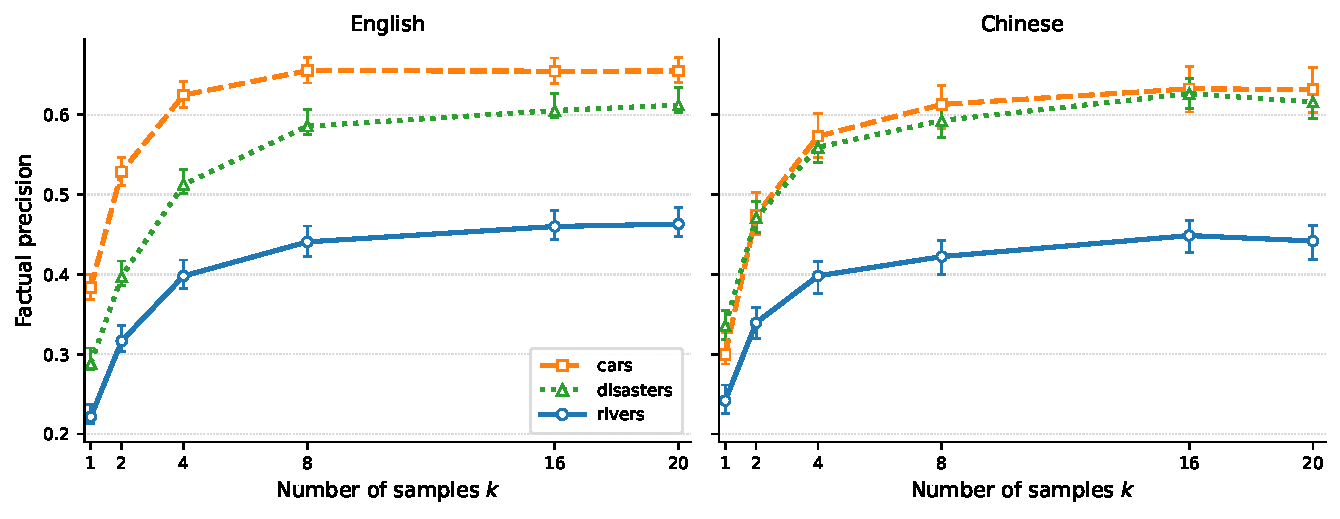
\includegraphics[width=\textwidth]{figures/prefix_scaling_en_zh.pdf}%
%   \caption{LLMAgg prefix scaling across sample budgets. Performance improves sharply at small $k$ and saturates by roughly $k=8$--$16$ in both languages, with only marginal changes beyond $k=20$.}
%   \label{fig:prefix_scaling}
% \end{figure*}

% \section{Experimental Setup}

% \paragraph{Dataset}

% Evaluating long-form factuality under long-tail conditions requires more than a standard entity benchmark. Popularity-aware resources such as PopQA provide valuable supervision for knowledge frequency, but they target short-answer question answering rather than long-form generation~\citep{popqa}. Long-form factuality benchmarks are closer to our setting, but they typically do not provide explicit domain splits together with controlled popularity partitions, which limits their usefulness for analyzing long-tail behavior in a structured way~\citep{wildhallucinations}.

% We therefore use RiDiC~\citep{braslavski2026chroniclesridicgeneratingdatasets}, a benchmark designed for entity-centric long-form factuality evaluation with explicit popularity stratification. RiDiC covers three domains (rivers, cars, and disasters) and two languages (English and Chinese). We report results on the test split only. The benchmark also provides popularity tiers---head, torso, and tail---derived from \texttt{popularity\_part\_sector}. This structure allows us to analyze not only average performance but also how factuality and adaptive inference behavior vary across common and rare entities.

% \paragraph{Generation}

% Our generator is Llama 3.1 8B Instruct\footnote{\url{hf.co/unsloth/Llama-3.1-8B-Instruct}}. We use temperature sampling to induce diversity across generations. In the full self-consistency setting, we sample 99 candidate completions per input. For readability, our prefix experiments report LLMAgg results at $\operatorname{K} \in \{1,2,4,8,16,20\}$. The $\operatorname{K}=99$ LLMAgg run serves as the full-budget reference for adaptivity, while $\operatorname{K}=20$ is used for the main prefix figure because the curves are already close to saturation by that point. Decoding settings are fixed across methods to ensure fair comparison.

% \paragraph{Compared Methods}

% We compare four main methods. \textbf{Single} uses one generated completion and performs no aggregation. \textbf{SeqProb} is a logprob-based selector baseline that chooses a candidate according to sequence probability. \textbf{Fact-majority} aggregates candidate responses by voting over FactOwl-derived atomic facts. \textbf{LLMAgg} uses a separate LLM call to synthesize a final response from multiple candidates. Unlike selection-based methods, it can combine complementary information across generations rather than choosing a single candidate.

% \paragraph{Evaluation}

% We use FactOwl as a fact-level evaluation framework that decomposes long-form outputs into atomic claims and estimates factual precision from their support status. We report factual precision as the main metric. Coverage and retention curves are computed from per-topic scoring outputs. In the main results, `Single` refers to the one-generation baseline, whereas `K=1` in the prefix table denotes the first prefix point of the self-consistency pipeline. These should not be expected to match exactly.

% \paragraph{Statistical Significance}

% We estimate uncertainty with bootstrap confidence intervals for the main metrics. For each setting, we resample test instances with replacement 1000 times and compute 95\% confidence intervals for factual precision, compute savings, and score retention.

% \paragraph{Adaptive Policy}

% To reduce inference cost, we train a simple input-only random forest that predicts an appropriate generation budget. Features include input length, punctuation, language, wh-patterns, domain indicators, and a baseline budget feature. The training protocol uses stratified shuffle splits with held-out test folds. The routing model only uses features available at inference time and therefore does not rely on label leakage. Feature importance is dominated by input length (about 0.31) and average word length (about 0.32), while domain and language features contribute less than 0.03. This indicates that the adaptive policy relies primarily on input complexity rather than domain identity.

% We intentionally use a simple model to isolate whether input-level signals alone are sufficient to capture variation in required compute.

% We report two main operating points, corresponding to retention targets of 0.95 and 0.99. We define \texttt{compute\_savings} as relative savings with respect to full-budget LLMAgg, \texttt{score\_retention} as the ratio between adaptive score and full-budget score, and `coverage` as the fraction of examples meeting the retention target.

% \section{Self-Consistency and Aggregation Results}

% \begin{table*}[htbp!]
% \centering
% \footnotesize
% \setlength{\tabcolsep}{2pt}
% \begin{adjustbox}{max width=\textwidth,center}
% \begin{tabular}{
% l l
% S[table-format=1.3]
% S[table-format=1.3]
% S[table-format=1.3]
% S[table-format=1.3]
% S[table-format=1.3]
% S[table-format=1.3]
% }
% \toprule
% \textbf{Lang} & \textbf{Domain} & 
% \textbf{Single} & \textbf{Best} & 
% \textbf{MC} & \textbf{MF} & 
% \textbf{SP} & \textbf{LLMAgg} \\
% \midrule

% \multirow{3}{*}{EN}
%  & rivers     & \bootcell{0.211}{0.012} & \bootcell{0.450}{0.015} & \bootcell{0.053}{0.014} & \bootcell{0.088}{0.008} & \multicolumn{1}{c}{0.233} & \bootcell{0.465}{0.019} \\
%  & cars       & \bootcell{0.344}{0.014} & \bootcell{0.622}{0.013} & \bootcell{0.218}{0.026} & \bootcell{0.146}{0.012} & \multicolumn{1}{c}{0.412} & \bootcell{0.656}{0.016} \\
%  & disasters  & \bootcell{0.283}{0.012} & \bootcell{0.574}{0.012} & \bootcell{0.112}{0.020} & \bootcell{0.111}{0.010} & \multicolumn{1}{c}{0.352} & \bootcell{0.619}{0.015} \\
% \midrule

% \multirow{3}{*}{ZH}
%  & rivers     & \bootcell{0.266}{0.018} & \bootcell{0.555}{0.019} & \bootcell{0.154}{0.027} & \bootcell{0.034}{0.007} & \multicolumn{1}{c}{0.233} & \bootcell{0.440}{0.021} \\
%  & cars       & \bootcell{0.344}{0.021} & \bootcell{0.640}{0.022} & \bootcell{0.216}{0.040} & \bootcell{0.019}{0.006} & \multicolumn{1}{c}{0.412} & \bootcell{0.632}{0.029} \\
%  & disasters  & \bootcell{0.355}{0.018} & \bootcell{0.707}{0.014} & \bootcell{0.234}{0.029} & \bootcell{0.031}{0.007} & \multicolumn{1}{c}{0.352} & \bootcell{0.616}{0.020} \\
% \bottomrule
% \end{tabular}%
% \end{adjustbox}
% \caption{Performance comparison across languages and domains. Cells show bootstrap mean $\pm$ half-width for methods with topic-level traces; \textbf{SP} is summary-only and has no bootstrap trace. \textbf{Single}: one generation, no aggregation. \textbf{Best}: best single candidate by factual precision. \textbf{MC}: majority co-occurrence voting. \textbf{MF}: majority fact-level voting. \textbf{SP}: SeqProb selection. \textbf{LLMAgg}: LLM-based aggregation ($k$=99).}
% \label{tab:results}
% \end{table*}

% % Table~\ref{tab:results} shows a clear and consistent pattern: \textbf{LLMAgg} is the strongest overall method across the benchmark. Relative to \textbf{Single}, it improves factual precision in every language--domain pair, with especially large gains on the more challenging settings. This trend holds for both English and Chinese, indicating that the benefit of aggregation is not confined to a single domain or language.

% % A more informative comparison is against stronger selection-based baselines. \textbf{SeqProb} improves over \textbf{Single}, but it remains well below \textbf{LLMAgg} in all reported settings. This suggests that the main advantage does not come from choosing a better individual completion, but from combining partially correct candidates and resolving contradictions across them. The same conclusion is supported by the fact-voting baselines: both \textbf{MC} and \textbf{MF} are consistently weaker than \textbf{LLMAgg}, implying that simple agreement-based aggregation is insufficient for this task.

% % In Chinese, \textbf{Best} remains a strong upper bound, and \textbf{LLMAgg} does not fully match it. In English, however, \textbf{LLMAgg} meets or exceeds \textbf{Best} across all three domains. This is a qualitatively important result: aggregation can produce summaries that are not only better than a typical single sample, but in some settings better than the best individual candidate in the pool. This behavior is consistent with the intuition behind LLMAgg, namely that long-form factuality benefits from consolidating complementary correct information rather than selecting one candidate wholesale.

% % Bootstrap uncertainty estimates support the robustness of these findings. For methods with topic-level traces, the intervals for \textbf{LLMAgg} are generally well separated from those of \textbf{Single}, and in many cases also from the simpler aggregation baselines. We therefore view the gains as systematic rather than anecdotal.

% % Overall, the results suggest that the effect of LLMAgg is broad and stable. It is not tied to a particular topic family, language, or narrow slice of the benchmark. Instead, the same pattern recurs across heterogeneous settings, which is exactly the behavior one would want from a method aimed at improving long-form factuality under controlled long-tail variation.

% \section{Self-Consistency and Aggregation Results}

% The central result is that aggregation, rather than sampling alone, is the main driver of factuality gains in this setting. Across all language-domain combinations, LLMAgg is the strongest method overall, consistently outperforming the raw single-sample baseline as well as weaker selection and voting alternatives.

% Two conclusions follow from Table~\ref{tab:results}. First, multi-sample inference is useful only when the sampled candidates are combined with a sufficiently strong aggregation mechanism. Selection-based baselines such as SeqProb improve over Single, but they remain substantially weaker than LLMAgg. Likewise, majority-style aggregation over completions or fact decisions fails to recover the same gains. This indicates that long-form factuality benefits less from choosing one ``best'' candidate than from consolidating partially correct information distributed across several candidates.

% Second, LLMAgg is robust across heterogeneous settings rather than being driven by a single favorable slice of the benchmark. The same ordering of methods recurs across both languages and all three domains, despite substantial differences in absolute difficulty. In English, LLMAgg even matches or exceeds the best individual candidate in the sampled pool, which suggests that synthesis can sometimes produce outputs that are stronger than any single completion viewed in isolation.

% Bootstrap intervals support the stability of this pattern. For methods with instance-level traces, the intervals for LLMAgg are generally well separated from those of Single and the weaker aggregation baselines. We therefore interpret the observed gains as systematic evidence that long-form factuality improves primarily through content-level consolidation rather than through simple response selection.

% \paragraph{Prefix Scaling}

% \begin{table}[htbp]
% \centering
% \small
% \setlength{\tabcolsep}{3pt}

% \resizebox{\linewidth}{!}{%
% \begin{tabular}{
% l l
% S[table-format=1.3]
% S[table-format=1.3]
% S[table-format=1.3]
% S[table-format=1.3]
% S[table-format=1.3]
% S[table-format=1.3]
% }
% \toprule
% \textbf{Lang} & \textbf{Domain} & \multicolumn{6}{c}{\textbf{$k$}} \\
% \cmidrule(lr){3-8}
%  & & \multicolumn{1}{c}{\textbf{1}} & \multicolumn{1}{c}{\textbf{2}} & \multicolumn{1}{c}{\textbf{4}} &
% \multicolumn{1}{c}{\textbf{8}} & \multicolumn{1}{c}{\textbf{16}} & \multicolumn{1}{c}{\textbf{20}} \\
% \midrule

% \multirow{3}{*}{EN}
%  & rivers     & 0.222 & 0.317 & 0.398 & 0.441 & 0.460 & 0.463 \\
%  & cars       & 0.384 & 0.529 & 0.625 & 0.655 & 0.655 & 0.655 \\
%  & disasters  & 0.289 & 0.397 & 0.513 & 0.586 & 0.605 & 0.612 \\

% \midrule

% \multirow{3}{*}{ZH}
%  & rivers     & 0.242 & 0.340 & 0.398 & 0.422 & 0.449 & 0.442 \\
%  & cars       & 0.300 & 0.474 & 0.573 & 0.613 & 0.633 & 0.632 \\
%  & disasters  & 0.335 & 0.471 & 0.559 & 0.593 & 0.627 & 0.616 \\

% \bottomrule
% \end{tabular}%
% }

% \caption{LLMAgg prefix curve at selected budgets ($k$). Point estimates are shown; bootstrap intervals are summarized in the Robustness Analysis paragraph.}
% \label{tab:prefix_curve}
% \end{table}

% % Table~\ref{tab:prefix_curve} and Figure~\ref{fig:prefix_scaling} report LLMAgg prefix curves for selected budgets. The main pattern is early saturation. In English cars, performance rises from $0.384$ at $k=1$ to 0.625 at $k=4$, with only marginal change thereafter (0.655 at $k=8$ and 0.655 at $k=20$). English disasters and rivers show the same qualitative behavior, with large early gains and much smaller improvements after $\bm{k}=8$ or $\bm{k}=16$. Chinese follows the same overall pattern.

% % This result matters for two reasons. First, it confirms that self-consistency is genuinely useful in this setting: increasing the prefix budget yields large factuality gains over very small budgets. Second, it shows that naive scaling is inefficient. The practical operating region is typically around $k=8$ to $16$, while additional samples beyond that range contribute only limited improvement. This observation directly motivates the use of adaptive sampling, as different inputs reach saturation at different budgets. We further compare $\operatorname{K}=20$ with larger budgets up to $\operatorname{K}=99$. The gap is negligible across all settings, ranging from $-0.0034$ to $0.0148$; for example, EN rivers changes from 0.4651 at $\operatorname{K}=20$ to 0.4617 at $\operatorname{K}=99$. In some settings, increasing $k$ slightly degrades performance, suggesting that excessive sampling can introduce noise rather than additional signal.

% % \paragraph{Prefix Scaling}

% Table~\ref{tab:prefix_curve} and Figure~\ref{fig:prefix_scaling} show a consistent early-saturation pattern. Factuality improves rapidly as the sample budget increases from very small values, but the marginal benefit declines sharply once the budget reaches a moderate range.

% This behavior has two implications. First, self-consistency is genuinely useful for long-form factual generation: moving from one or two samples to a small multi-sample pool yields large gains in every setting we evaluate. Second, naive test-time scaling is inefficient. In most cases, the practical operating region is around $k=8$--$16$, after which additional samples contribute little and occasionally even reduce performance slightly. This non-monotonicity suggests that larger candidate pools can introduce noise or reinforce erroneous content rather than consistently adding new factual signal.

% The comparison between $\operatorname{K}=20$ and larger budgets up to $\operatorname{K}=99$ reinforces the same conclusion. The score differences in this range are negligible, which means that the full-budget reference is empirically very close to the prefix regime already shown in Table~\ref{tab:prefix_curve}. Taken together, these results motivate adaptive budget allocation: if most gains are realized early, then a fixed large budget is unlikely to be compute-efficient for all inputs.

% \paragraph{Popularity-Tier Analysis}


% \begin{table}[t]
% \centering
% \small
% \setlength{\tabcolsep}{4pt}

% \resizebox{\linewidth}{!}{%
% \begin{tabular}{
% l l l
% S[table-format=1.3]
% S[table-format=1.3]
% S[table-format=1.3]
% }
% \toprule
% \textbf{Lang} & \textbf{Domain} & \textbf{Tier} &
% \textbf{Single} & \textbf{LLMAgg@20} & $\boldsymbol{\Delta}$ \\
% \midrule

% \multirow{9}{*}{EN}
%  & \multirow{3}{*}{rivers}
%    & head  & 0.429 & 0.837 & 0.408 \\
%  &        & torso & 0.322 & 0.676 & 0.354 \\
%  &        & tail  & 0.160 & 0.363 & 0.204 \\

%  & \multirow{3}{*}{cars}
%    & head  & 0.458 & 0.863 & 0.406 \\
%  &        & torso & 0.450 & 0.815 & 0.365 \\
%  &        & tail  & 0.299 & 0.580 & 0.281 \\

%  & \multirow{3}{*}{disasters}
%    & head  & 0.448 & 0.783 & 0.336 \\
%  &        & torso & 0.379 & 0.796 & 0.417 \\
%  &        & tail  & 0.270 & 0.596 & 0.326 \\

% \midrule

% \multirow{9}{*}{ZH}
%  & \multirow{3}{*}{rivers}
%    & head  & 0.510 & 0.749 & 0.239 \\
%  &        & torso & 0.344 & 0.550 & 0.206 \\
%  &        & tail  & 0.202 & 0.355 & 0.152 \\

%  & \multirow{3}{*}{cars}
%    & head  & 0.435 & 0.771 & 0.336 \\
%  &        & torso & 0.389 & 0.689 & 0.300 \\
%  &        & tail  & 0.295 & 0.559 & 0.264 \\

%  & \multirow{3}{*}{disasters}
%    & head  & 0.495 & 0.750 & 0.256 \\
%  &        & torso & 0.456 & 0.785 & 0.329 \\
%  &        & tail  & 0.329 & 0.590 & 0.261 \\

% \bottomrule
% \end{tabular}%
% }

% \caption{Performance by frequency tier (head, torso, tail). $\Delta$ denotes the gain from \textbf{Single} to \textbf{LLMAgg@20}. Point estimates are shown; bootstrap intervals are summarized in the Robustness Analysis paragraph.}
% \label{tab:tier_results}
% \end{table}

% % Table~\ref{tab:tier_results} compares Single and LLMAgg@20 by popularity tier. Two patterns stand out. First, tail entities remain the weakest regime overall. Across languages and domains, head examples are typically easiest, torso examples are intermediate, and tail examples are hardest. This is consistent with the long-tail motivation of RiDiC.

% % Second, LLMAgg improves all tiers. In English rivers, the score jumps from 0.4293 to 0.8373 on head and from 0.1595 to 0.3634 on tail. In English cars, tail entities improve from 0.2987 to 0.5799 (+0.2812), while in Chinese disasters tail improves from 0.3292 to 0.5903 (+0.2611). Rivers show smaller gains than cars, consistent with the adaptive results: EN rivers save only 6.12\% compute at the 0.95 retention target, compared with 28.72\% for EN cars, suggesting lower redundancy and more gradual aggregation gains. These results do not support a single universal claim such as ``the gain is always largest on tail.'' Instead, the safer and more accurate conclusion is that LLMAgg improves factuality across all popularity tiers, while tail remains the hardest subset overall.

% % This tier analysis also clarifies the role of long-tail evaluation in our paper. Our claim is not that self-consistency completely closes the gap between head and tail. Rather, self-consistency materially improves long-form factuality even in the hardest regime, which is precisely where reliable generation is most needed.

% Table~\ref{tab:tier_results} shows that popularity remains a strong source of difficulty even under improved inference. Across languages and domains, tail entities are consistently the weakest regime, head entities are generally the strongest, and torso examples lie in between. Self-consistency therefore does not eliminate the long-tail problem.

% At the same time, LLMAgg improves performance in every popularity tier. This is important because it shows that the method is not merely exploiting easy high-frequency cases: the gains extend to the hardest long-tail subset as well. The size of the gain varies across domains and tiers, but the qualitative pattern is stable. The appropriate conclusion is therefore not that aggregation helps only on tail entities, nor that it closes the head--tail gap, but that it delivers broad factuality improvements while preserving the benchmark's underlying difficulty structure.

% This distinction matters for the interpretation of our results. The contribution of adaptive self-consistency is not to remove long-tail difficulty altogether, but to improve factual precision even when knowledge is sparse and entity frequency is low.

% \paragraph{Adaptive Budgeting}

% \begin{table}[t]
% \centering
% \small
% \setlength{\tabcolsep}{3pt}
% \resizebox{\linewidth}{!}{%
% \begin{tabular}{
% l l
% S[table-format=1.3]
% S[table-format=1.3]
% S[table-format=1.3]
% S[table-format=1.3]
% S[table-format=1.3]
% S[table-format=1.3]
% }
% \toprule
% \textbf{Lang} & \textbf{Domain} &
% \multicolumn{3}{c}{\textbf{Retention 0.95}} &
% \multicolumn{3}{c}{\textbf{Retention 0.99}} \\
% \cmidrule(lr){3-5} \cmidrule(lr){6-8}
% & & {\textbf{Savings}} & {\textbf{Retention}} & {\textbf{Coverage}} &
% {\textbf{Savings}} & {\textbf{Retention}} & {\textbf{Coverage}} \\
% \midrule
%   \multirow{3}{*}{EN}
%    & rivers     & 0.061 & 0.997 & 0.964 & 0.046 & 0.997 & 0.971 \\
%    & cars       & 0.287 & 0.994 & 0.850 & 0.135 & 0.994 & 0.914 \\
%    & disasters  & 0.179 & 1.004 & 0.903 & 0.088 & 1.012 & 0.938 \\
%   \midrule
%   \multirow{3}{*}{ZH}
%    & rivers     & 0.021 & 1.000 & 0.986 & 0.029 & 0.997 & 0.976 \\
%    & cars       & 0.156 & 1.022 & 0.912 & 0.055 & 1.016 & 0.965 \\
%    & disasters  & 0.115 & 1.001 & 0.936 & 0.062 & 1.000 & 0.954 \\

% \bottomrule
% \end{tabular}%
% }
% \caption{Adaptive retention-compute tradeoff at two retention targets. \textbf{Savings}: relative compute reduction vs.\ full-budget LLMAgg. \textbf{Retention}: ratio of adaptive to full-budget score. \textbf{Coverage}: fraction of examples meeting the retention target. Point estimates are shown; bootstrap intervals are summarized in the Robustness Analysis paragraph.}
% \label{tab:adaptive}
% \end{table}

% Formally, we define score retention as $\text{Retention} = \frac{\text{Fact}(\hat{y}_{\text{adaptive}})}{\text{Fact}(\hat{y}_{\text{full}})}$.

% \begin{figure*}[htbp]
%   \centering
%   \IfFileExists{figures/adaptive_tradeoff_scatter.pdf}{%
%     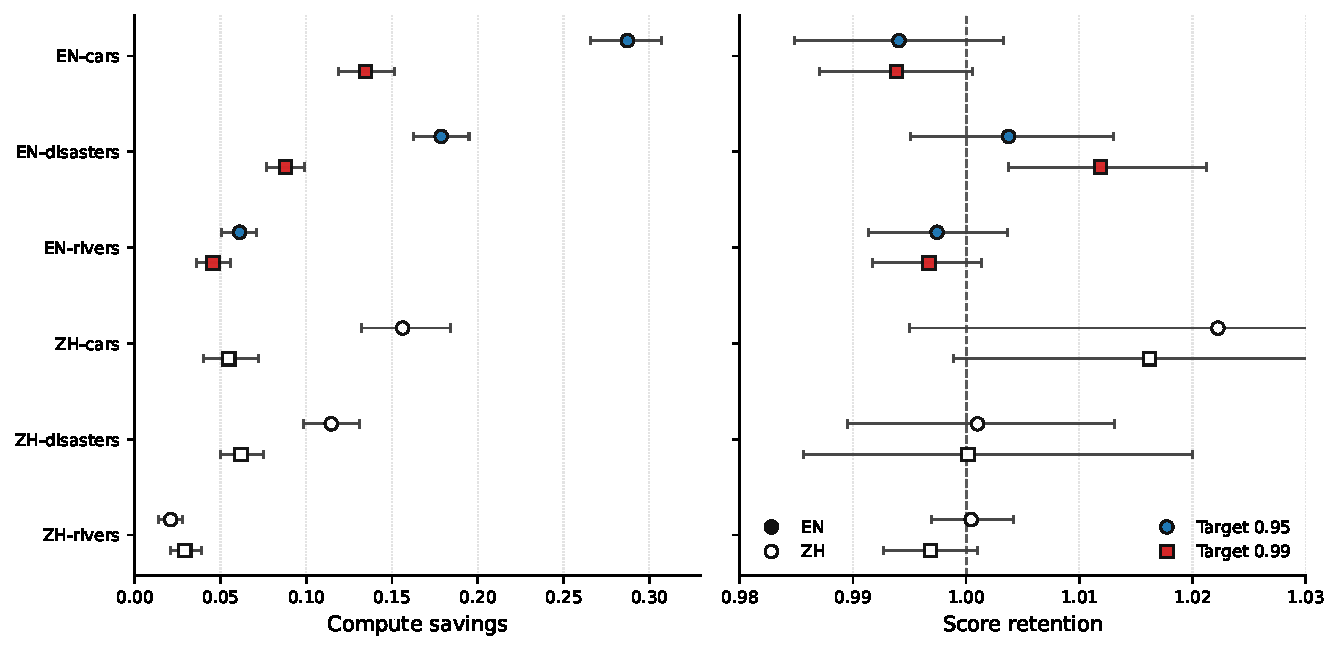
\includegraphics[width=\linewidth]{figures/adaptive_tradeoff_scatter.pdf}%
%   }{%
%     \fbox{\parbox{0.92\linewidth}{\centering Adaptive tradeoff figure placeholder.}}%
%   }
%   \caption{Adaptive inference tradeoff across domains and languages. Cars and disasters admit larger compute savings, while rivers remain harder to compress. Score retention remains close to full-budget performance in most settings.}
%   \label{fig:adaptive_tradeoff}
% \end{figure*}

% Table~\ref{tab:adaptive} and Figure~\ref{fig:adaptive_tradeoff} show that most of the full-budget benefit can be preserved without using a fixed large sampling budget for every input. The adaptive controller achieves score retention close to the full-budget reference across all settings, while reducing generation cost by an amount that depends strongly on domain.

% The key pattern is heterogenity. Cars and disasters admit meaningful compression, whereas rivers are much harder to compress aggressively. This matches the prefix-scaling results: when gains saturate quickly, adaptive routing has more freedom to reduce compute; when the curve is flatter and improvements accumulate more gradually, the room for savings is smaller. The adaptive results therefore do not simply demonstrate that routing works, but also reveal that the value of additional samples is domain-dependent.

% A second point is that high score retention does not imply uniform per-instance behavior. Coverage is lower in some settings, especially English cars at the looser target, indicating that a non-trivial minority of examples still fall below the desired retention threshold. In other words, adaptive routing is effective on average, but its benefits are not distributed uniformly across all inputs. This is consistent with the broader picture of the paper: inference-time compute is useful, but its payoff depends strongly on input difficulty.

% Finally, score retention slightly above 1.0 in some cells should not be interpreted as a contradiction. Because aggregation is not strictly monotonic in the number of candidates, a smaller routed budget can occasionally yield a marginally better final output than the nominal full-budget reference. Empirically, however, these deviations are small; the main result is that adaptive routing recovers nearly all of the full-budget gain while avoiding unnecessary sampling on many inputs.

% % Figure~\ref{fig:adaptive_tradeoff} complements Table~\ref{tab:adaptive} by visualizing the retention--compute tradeoff across domains and operating points.

% % Table~\ref{tab:adaptive} and Figure~\ref{fig:adaptive_tradeoff} report the adaptive retention-compute tradeoff. At the 0.95 retention target, the adaptive policy preserves almost all of the score while reducing compute in all domain-language pairs. The savings are largest for cars: 28.72\% in English and 15.62\% in Chinese. Disasters also admit meaningful savings, while rivers are harder to compress aggressively, especially in Chinese (2.10\% savings). Bootstrap intervals show that these savings are stable; for example, in English cars at the 0.95 target, compute savings are 0.2872 [0.2660, 0.3073] and score retention is 0.9941 [0.9848, 1.0033], while English disasters slightly exceed the full-budget score at 1.0038 [0.9951, 1.0131]. Smaller savings on rivers suggest that this domain requires more consistent sampling to stabilize factual outputs.

% % At the stricter 0.99 retention target, the policy becomes more conservative but still yields measurable savings. This is the expected pattern: as the retention target increases, the controller has less freedom to reduce budget, and compute savings shrink accordingly. Importantly, the score-retention values remain extremely close to 1.0 in both settings, showing that the adaptive controller recovers most of the benefit of full-budget LLMAgg.

% % These results give a practical interpretation of the prefix-scaling findings. Full-budget self-consistency is unnecessary for most inputs. Many examples saturate well before 99 samples, and a lightweight input-only controller can exploit this heterogeneity to reduce compute while preserving factuality. We note that LLMAgg introduces an additional aggregation call per input. However, this cost is constant with respect to $\operatorname{K}$ and does not affect relative compute savings from reducing the number of sampled generations. Even moderate savings are meaningful in long-form generation, where each additional sample incurs non-trivial cost.

% \paragraph{Qualitative Analysis}

% \begin{table*}[t]
% \centering
% \small
% \setlength{\tabcolsep}{4pt}

% \begin{tabular}{
% l l l l
% S
% S
% l
% }
% \toprule
% \textbf{Lang} & \textbf{Domain} & \textbf{Tier} & \textbf{Topic} &
% \textbf{Single} & \textbf{LLMAgg@20} & $\boldsymbol{\Delta}$ \\
% \midrule

% \multicolumn{7}{c}{\textit{Wins (LLMAgg improves over Single)}} \\
% \midrule

% EN & cars      & tail  & Jiotto Caspita                & 0.335 & 0.750 & \pos{0.415} \\
%    &           & head  & GAZelle                       & 0.546 & 0.929 & \pos{0.382} \\
%    & disasters & torso & Super Outbreak                & 0.455 & 0.900 & \pos{0.445} \\
%    &           & torso & Zanclean flood                & 0.509 & 0.917 & \pos{0.408} \\
%    & rivers    & head  & Blue Nile                     & 0.513 & 0.938 & \pos{0.424} \\
%    &           & torso & St.\ Marys River              & 0.424 & 0.813 & \pos{0.389} \\

% ZH & cars      & tail  & 劳斯莱斯 Silver Wraith        & 0.551 & 1.000 & \pos{0.449} \\
%    &           & tail  & 速霸陸 Alcyone                & 0.570 & 0.909 & \pos{0.339} \\
%    & disasters & tail  & 2016 緬甸地震                 & 0.523 & 0.933 & \pos{0.411} \\
%    &           & tail  & 飓风菲乔                       & 0.395 & 0.779 & \pos{0.384} \\
%    & rivers    & tail  & 馬伊默卡河                     & 0.278 & 0.800 & \pos{0.522} \\
%    &           & tail  & 巴科伊河                       & 0.340 & 0.818 & \pos{0.478} \\

% \midrule
% \multicolumn{7}{c}{\textit{Failures (LLMAgg degrades performance)}} \\
% \midrule

% EN & cars      & torso & Aston Martin Lagonda          & 0.583 & 0.267 & \nega{0.316} \\
%    &           & tail  & Audi S1                       & 0.819 & 0.450 & \nega{0.369} \\
%    & disasters & tail  & Hurricane Debby               & 0.548 & 0.000 & \nega{0.548} \\
%    &           & tail  & 2014 Mount Everest avalanche  & 0.828 & 0.279 & \nega{0.549} \\
%    & rivers    & tail  & Miass                         & 0.379 & 0.000 & \nega{0.379} \\
%    &           & tail  & Tsitsikamma River             & 0.674 & 0.235 & \nega{0.438} \\

% ZH & cars      & tail  & 三菱戈蓝拉姆达 / 普利茅斯札幌   & 0.647 & 0.147 & \nega{0.500} \\
%    &           & head  & 三菱日蝕                       & 0.704 & 0.065 & \nega{0.639} \\
%    & disasters & torso & 2024年花蓮地震                 & 0.837 & 0.097 & \nega{0.740} \\
%    &           & head  & 飓风海伦妮                     & 0.788 & 0.000 & \nega{0.788} \\
%    & rivers    & head  & 伏尔塔瓦河                     & 0.850 & 0.294 & \nega{0.556} \\
%    &           & head  & 卢比孔河                       & 0.990 & 0.368 & \nega{0.622} \\

% \bottomrule
% \end{tabular}

% \caption{
% Representative win and failure cases. $\Delta$ denotes the change from \textbf{Single} to \textbf{LLMAgg@20}. 
% Gains typically arise from aggregating complementary evidence across generations, 
% while failures are driven by consistent hallucinations, especially for ambiguous long-tail entities.
% }
% \label{tab:examples}
% \end{table*}

% % To better understand when LLMAgg helps and when it fails, we examine representative wins and losses in Table~\ref{tab:examples}. We identify two main patterns. First, successful cases arise when correct information is distributed across multiple candidates and can be consolidated by aggregation. LLMAgg can then synthesize a stronger final answer than any single candidate. Examples include Jiotto Caspita in English cars, Blue Nile in English rivers, and several Chinese tail examples such as 馬伊默卡河 and 巴科伊河.

% % We categorize errors into two main types: repeated hallucinations, where incorrect facts are consistently present across multiple samples and reinforced by aggregation, and entity ambiguity, where multiple plausible interpretations lead to unstable aggregation outcomes. This can produce dramatic drops, as seen for Hurricane Debby (0.5475 to 0.0000), 2024年花蓮地震 (0.8369 to 0.0970), and several high-scoring head examples in Chinese. Failing cases also tend to start from stronger single-sample outputs: in English, failures average 0.64 versus 0.58 for successful cases, and the failing inputs are slightly longer on average (73 versus 70 characters).

% % These cases suggest that aggregation is powerful but not uniformly safe. Its main benefit is to combine dispersed correct information, while its main risk is to amplify repeated misinformation. This also explains why adaptive routing is useful: if some inputs are already easy or already unstable, spending more compute on them may not always be the best strategy.

% % These observations suggest that aggregation benefits from diversity only when correct information is present in the candidate pool.

% The qualitative examples in Table~\ref{tab:examples} clarify both the strengths and the risks of aggregation. Successful cases typically arise when correct information is fragmented across several candidates: no individual completion is fully reliable, but the pooled sample set contains enough complementary evidence for LLMAgg to construct a stronger final answer. In this regime, aggregation acts as a synthesis mechanism rather than a selector.

% Failure cases follow a different logic. We observe two recurrent error modes. The first is repeated hallucination: the same unsupported content appears across multiple samples and is therefore reinforced rather than removed during aggregation. The second is entity ambiguity, where multiple plausible referents or unstable interpretations make it difficult for the aggregator to identify a consistent factual core. In both cases, adding more samples can actually strengthen the wrong consensus.

% These examples help explain the broader empirical results. Aggregation is powerful when the candidate pool contains diverse but recoverable factual signal, and much less reliable when the pool is dominated by correlated errors. This also provides a rationale for adaptive routing: the value of additional samples depends not only on how much diversity they introduce, but also on whether that diversity contains usable factual information.

% % \paragraph{Robustness Analysis}

% % We analyze robustness using the bootstrap estimates above. Across domains and languages, LLMAgg consistently outperforms Single and the weaker baselines, and all LLMAgg improvements over Single are statistically significant under bootstrap resampling. Prefix-scaling trends remain consistent under resampling, with early saturation observed in all settings.

% % The adaptive policy is also stable under bootstrap resampling. At the 0.95 retention target, compute savings remain substantial while score retention stays very close to 1.0. In particular, English cars retain 0.9941 [0.9848, 1.0033] of the full-budget score while saving 0.2872 [0.2660, 0.3073] of compute. As an additional baseline, ReASC fails to improve over Single in all settings, despite using 12.852 samples on average for EN cars and 18.160 for ZH cars; the corresponding scores remain 0.3446 versus 0.3446 and 0.3418 versus 0.3418, respectively, so the baseline is numerically indistinguishable from Single at the reported precision. This suggests that shallow early stopping signals are insufficient for long-form factuality.


% \paragraph{Robustness Analysis}

% The main empirical trends remain stable under bootstrap resampling. Across domains and languages, LLMAgg consistently remains above Single and the weaker baselines, and the prefix-scaling curves preserve the same rapid-gain--then-saturation shape. This strengthens the interpretation that the results reflect a stable property of the evaluation setting rather than noise in a few benchmark slices.

% The adaptive results are similarly stable. Score retention remains close to the full-budget reference across resamples, while compute savings retain the same domain-dependent structure discussed above. In particular, the contrast between more compressible domains such as cars and less compressible ones such as rivers persists under resampling, suggesting that this heterogeneity is genuine rather than an artifact of a single split.

% As an additional point of reference, ReASC fails to improve meaningfully over Single despite using a non-trivial number of samples on average. This contrast suggests that early stopping by itself is insufficient in long-form factual generation unless it is paired with an aggregation mechanism capable of exploiting complementary evidence across samples.

% \section{Discussion}

% \paragraph{Takeaway 1: Self-consistency helps, but aggregation is the key mechanism.}
% Across domains and languages, multi-sample inference substantially improves long-form factuality only when paired with a strong aggregation strategy. LLMAgg consistently outperforms weaker baselines such as SeqProb and fact-majority, suggesting that the main benefit comes from consolidating partially correct information across samples rather than selecting a single high-probability response.

% \paragraph{Takeaway 2: The gains saturate early.}
% Prefix-scaling results show that most factuality improvements are achieved at moderate budgets, typically around $k=8$--$16$. Beyond this range, additional samples yield only marginal benefit and may even introduce noise. This indicates that inference-time scaling for factuality is useful, but not in a naive fixed-budget form.

% \paragraph{Takeaway 3: Adaptive budgeting is practically viable, but heterogeneous across domains.}
% A simple input-only controller retains most of the full-budget gain while reducing compute, especially in cars and disasters. Rivers are harder to compress, suggesting that some domains require more consistent sampling to stabilize factual outputs. The practical implication is that budget allocation should depend on input difficulty rather than be fixed uniformly.

% \paragraph{Takeaway 4: Long-tail factuality remains difficult even with stronger inference.}
% Tail entities remain the hardest regime overall, and aggregation is not uniformly safe. When the candidate pool contains repeated hallucinations or ambiguous entity interpretations, aggregation can amplify errors rather than correct them. This suggests that the remaining bottleneck is not only model knowledge, but also the reliability with which inference-time procedures can extract and consolidate correct information under sparse long-tail conditions.

% \section*{Limitations}

% This study has several limitations. First, the reported results are centered on one generator family. Second, the adaptive policy is intentionally simple and uses only input-level features. Third, we do not claim that the selected budgets are universally optimal outside this setting. Fourth, multilingual factuality evaluation inevitably contains some evaluator noise, especially in more difficult or ambiguous cases.

% Finally, we do not explore alternative aggregation architectures beyond LLM prompting.

% \section{Conclusion}

% We presented a study of adaptive self-consistency for long-form factuality under explicit long-tail conditions. Across domains and languages, LLM-based aggregation substantially improves over single generation and weaker aggregation baselines. Prefix-scaling experiments show that most gains appear at moderate budgets, and an input-only adaptive policy retains nearly all of the full-budget benefit while reducing compute. These results suggest that self-consistency is a strong tool for long-form factuality, but that its practical deployment should be budget-aware rather than fixed-budget.

% \bibliography{custom}

% \appendix
% \section{Supplementary Material}

% \subparagraph*{Notes}
% \begin{itemize}
%     \item The current implementation uses the model tokenizer chat template, so the exact serialized prompt depends on the chosen base model.
%     \item The English and Chinese templates differ only in language and marker string.
%     \item The marker strings are:
%     \begin{itemize}
%         \item English: \texttt{Final Consolidated Answer:}
%         \item Chinese: \texttt{最终整合后的答案：}
%     \end{itemize}
% \end{itemize}

% \clearpage
% \paragraph{LLMAgg Prompt Templates}

% The prompt bodies below are the exact LLMAgg templates used in the current RiDiC pipeline. The final prompt is assembled with the model chat template, so the effective input includes the system prompt, instruction block, user question, and the candidate answers formatted as \verb|### Answer N|.

% \begin{figure*}[p]
% \centering
% \begin{minipage}{0.98\textwidth}
% \begin{PromptBox}{English LLMAgg Prompt Template}
% \textbf{System prompt}

% You are an Answer Aggregator. Your task is to read several candidate answers to the same question and produce ONE coherent, high-quality answer.

% \medskip
% \textbf{Instructions}
% \begin{itemize}
%   \item Follow these rules exactly:
%   \item Identify the main points made in each candidate answer.
%   \item Keep every point that appears in a majority of the answers (>= half).
%   \item Add complementary details that are already present in the existing answers and do not contradict the majority view.
%   \item When answers disagree, choose the version supported by the majority. If tied, pick the clearer or more detailed wording.
%   \item Rewrite everything into a single, well-structured response.
%   \item Do not mention the aggregation process, voting, or the existence of other answers.
% \end{itemize}

% \medskip
% \textbf{Output format (nothing else):}

% Final Consolidated Answer:
% [your aggregated answer]

% \medskip
% \textbf{User prompt template}

% Question:
% \verb|{question}|

% Candidate Answers (delimited by \verb|###|):
% \verb|### Answer 1|
% \verb|{answer_1}|
% \verb|### Answer 2|
% \verb|{answer_2}|
% ...
% \verb|### Answer k|
% \verb|{answer_k}|

% End of input.
% \end{PromptBox}
% \end{minipage}
% \end{figure*}

% \begin{figure*}[p]
% \centering
% \begin{minipage}{0.98\textwidth}
% \begin{PromptBox}{Chinese LLMAgg Prompt Template}
% \textbf{System prompt}

% 你是一名答案聚合器。你的任务是阅读同一问题的多个候选答案，并输出一个连贯且高质量的最终答案。

% \medskip
% \textbf{Instructions}
% \begin{itemize}
%   \item 严格遵循以下规则：
%   \item 找出每个候选答案中的关键信息点。
%   \item 保留在大多数答案中出现的要点（>= 一半）。
%   \item 可以加入候选答案中已有且不与多数观点冲突的补充细节。
%   \item 当答案不一致时，选择由多数支持的版本；若持平，选择更清晰或更详细的表述。
%   \item 将内容重写为一个结构良好的单一回答。
%   \item 不要提及聚合过程、投票或其他答案的存在。
% \end{itemize}

% \medskip
% \textbf{Output format (且仅输出该格式):}

% 最终整合后的答案：
% [你的整合答案]

% \medskip
% \textbf{User prompt template}

% 问题:
% \verb|{question}|

% 候选答案（以 \verb|###| 分隔）:
% \verb|### Answer 1|
% \verb|{answer_1}|
% \verb|### Answer 2|
% \verb|{answer_2}|
% ...
% \verb|### Answer k|
% \verb|{answer_k}|

% 输入结束。
% \end{PromptBox}
% \end{minipage}
% \end{figure*}

% \section{RiDiC and FactOwl Details}

% \paragraph{RiDiC Benchmark}

% RiDiC is a benchmark for long-form factuality evaluation designed 
% to assess model performance on entity-centric generation tasks 
% under controlled popularity conditions. The benchmark covers three 
% domains: rivers, cars, and natural disasters, and includes data in 
% two languages: English and Chinese.

% A key feature of RiDiC is the explicit stratification of entities 
% into popularity tiers: head, torso, and tail. These tiers correspond 
% to different levels of entity frequency and availability in training 
% data, enabling systematic analysis of model performance in long-tail 
% settings.

% Each instance in RiDiC consists of an entity prompt $x$ and a generated 
% response $y$. The response is a long-form text containing multiple 
% factual statements. This distinguishes RiDiC from short-answer 
% benchmarks, as errors may occur at the level of individual facts 
% within an otherwise coherent response.

% \paragraph{FactOwl Evaluation Framework}

% We evaluate factuality using FactOwl, a framework for fine-grained 
% fact-level verification of generated text. Given a model output $y$, 
% FactOwl decomposes it into a set of atomic factual statements:
% \begin{equation}
%     F(y) = \{f_1, f_2, \dots, f_n\}.    
% \end{equation}


% Each fact $f_i$ is independently verified against external knowledge 
% sources, resulting in a binary support indicator:
% \begin{equation}
% \mathbb{1}(f_i) =
% \begin{cases}
% 1, & \text{if } f_i \text{ is supported}, \\
% 0, & \text{otherwise}.
% \end{cases}
% \end{equation}

% The factuality score of a response $y$ is then defined as:
% \begin{equation}
%     \text{Fact}(y) = \frac{1}{|F(y)|} \sum_{f_i \in F(y)} \mathbb{1}(f_i).
% \end{equation}

% This formulation captures partial correctness of long-form outputs, 
% allowing both correct and incorrect statements to contribute to the 
% final score. The approach is conceptually similar to FActScore 
% \citep{min-etal-2023-factscore}, but adapted to the RiDiC setting.

% \paragraph{Self-Consistency and Aggregation}

% In the self-consistency setting, we sample $\operatorname{K}$ independent responses
% from the model:
% \begin{equation}
%     y^{(1)}, y^{(2)}, \dots, y^{(K)} \sim p_\theta(y \mid x).
% \end{equation}

% An aggregation function $\mathcal{A}$ is then applied to produce a 
% final response:
% \begin{equation}
%     \hat{y} = \mathcal{A}\left(y^{(1)}, \dots, y^{(K)}\right).
% \end{equation}

% We evaluate the factuality of the aggregated output using the same 
% fact-level metric:
% \begin{equation}
%     \text{Fact}(\hat{y}).
% \end{equation}


% This setup allows us to study how aggregation strategies influence 
% factual correctness in long-form generation.

% \paragraph{Adaptive Inference}

% To reduce computational cost, we consider adaptive inference strategies 
% that vary the number of samples $\operatorname{K}$ per input. Instead of using a fixed
% budget, we predict a suitable value $\operatorname{K} = g(x)$ using a classifier
% based on features of the input or intermediate generations:
% \begin{equation}
%     K = g(x),    
% \end{equation}
% where $g$ is a learned model.

% The final output is then computed as:
% \begin{equation}
%     \hat{y} = \mathcal{A}\left(y^{(1)}, \dots, y^{(K)}\right).    
% \end{equation}


% This formulation enables trading off computational cost and factuality by allocating more samples to difficult inputs while keeping inference efficient overall.

% \paragraph{Adaptive Feature Importance}

% Feature importance for the adaptive controller is dominated by input length and lexical-complexity features, while language and domain indicators contribute relatively little. This suggests that the controller relies primarily on input complexity rather than domain identity.

% \begin{figure*}[t]
%   \centering
%   \IfFileExists{figures/adaptive_feature_importance.pdf}{%
%     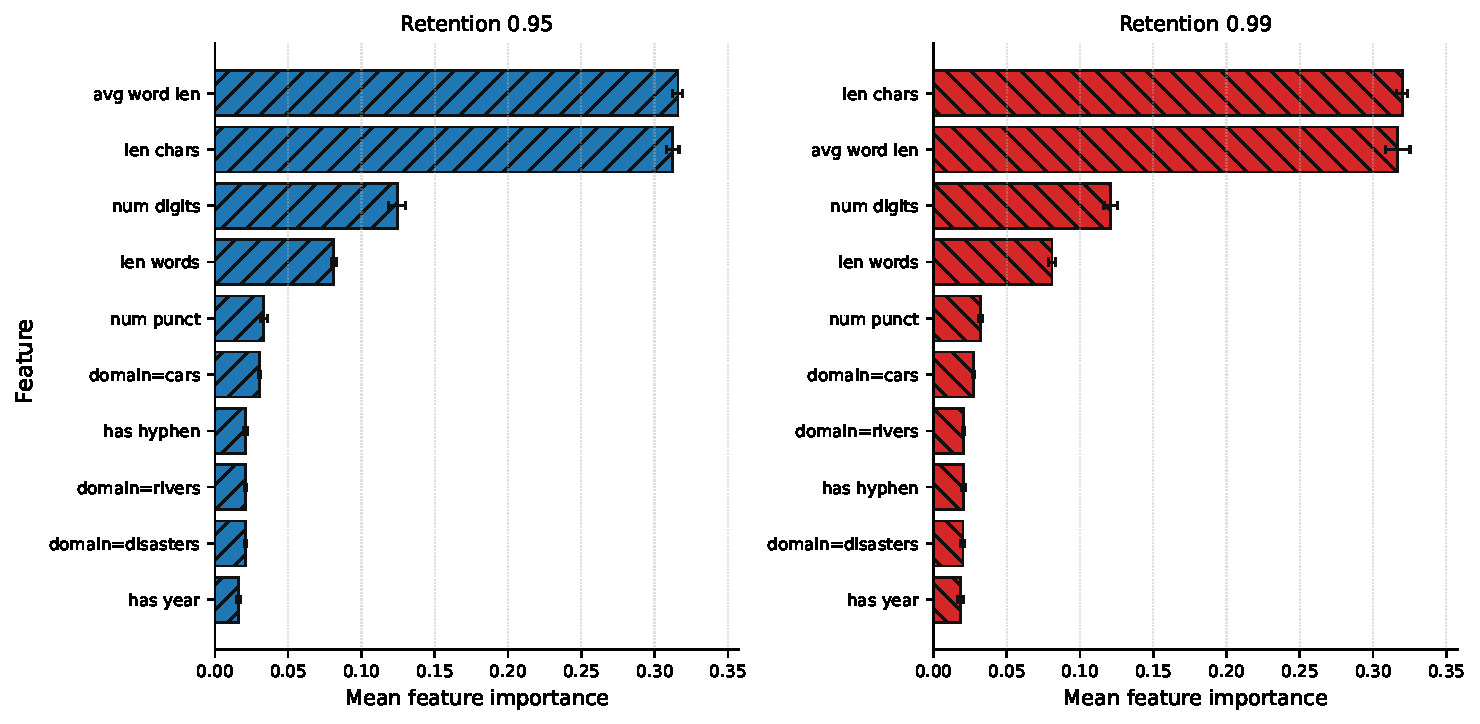
\includegraphics[width=\textwidth]{figures/adaptive_feature_importance.pdf}%
%   }{%
%     \fbox{\parbox{0.92\textwidth}{\centering Adaptive feature-importance figure placeholder.}}%
%   }
%   \caption{Feature importance for the adaptive controller. Input length and lexical-complexity features dominate, while language and domain indicators contribute relatively little. Error bars show the standard deviation of feature importance across runs.}
%   \label{fig:feature_importance}
% \end{figure*}

% \paragraph{Examples from RiDiC}

% Table~\ref{tab:ridicexample} presents an example from the RiDiC benchmark, illustrating the variability and factual inconsistencies in model outputs.

% \begin{table*}[t]
% \small
% \centering
% \begin{tabular}{p{0.95\textwidth}}
% \toprule
% \textbf{Entity:} Xiaomi SU7 \\
% \midrule

% \textbf{Model Output A (hallucinated):}  
% The Xiaomi SU7 is a subcompact SUV based on the SAIC MG ZS platform, 
% featuring a 1.5-liter engine and manual transmission. \\

% \textbf{Model Output B (partially correct):}  
% The Xiaomi SU7 is an electric SUV launched in 2022, offering a range 
% of up to 600 km and competing with vehicles such as the Tesla Model Y. \\

% \textbf{Model Output C (more accurate):}  
% The Xiaomi SU7 is an all-electric sedan unveiled in 2023, built on 
% Xiaomi's proprietary platform, with high-performance variants exceeding 
% 600 horsepower and long driving range. \\

% \midrule

% \textbf{Example Facts:}
% \begin{itemize}
%     \item The Xiaomi SU7 is an electric vehicle. \hfill (True)
%     \item It is a subcompact SUV based on MG ZS. \hfill (False)
%     \item It was unveiled in 2023. \hfill (True)
%     \item It has a 1.5L combustion engine. \hfill (False)
%     \item It competes with Tesla Model Y. \hfill (Partially True)
% \end{itemize}
% \\
% \bottomrule
% \end{tabular}
% \caption{Example from RiDiC showing inconsistent generations for the same entity.}
% \label{tab:ridicexample}
% \end{table*}

% This example motivates aggregation, which aims to preserve consistent facts across samples while removing unsupported claims.

% \paragraph{Prompt Robustness}

% We tested minor variations of the aggregation prompt and did not observe material changes in LLMAgg performance, suggesting that the results are not highly sensitive to prompt wording.

% \end{document}
